\chapter{Анализ производительности опорной беспроводной сети}\label{ch:ch4}
Беспроводные сети часто используются для создания опорных сетей на больших расстояниях, особенно когда проводная сеть недоступна по тем или иным причинам. Для построения опорных сетей часто используются радиорелейное оборудование или радиомаршрутизаторы стандарта IEEE 802.11 (WiFi) или IEEE 802.16 (WiMax).

Одна из отличительных черт беспроводных сетей с множественным доступом "--- сложные методы доступа к каналу. В беспроводной сети с множественным доступом к каналу одновременно может быть подключено несколько станций, причем некоторые станции могут не слышать друг друга (проблема скрытых станций). Из-за этого возникают ситуации, когда две или более станций ведут одновременные передачи, которые искажаются на приемнике и возникают коллизии. Кроме того, передачи сигналов в беспроводных сетях значительно больше подвержены искажениям из-за многолучевого распространения сигнала, движения станций, изменений условий окружающей среды и других факторов. По этим причинам в беспроводных сетях с множественным доступом (в том числе, в сетях IEEE 802.11 и IEEE 802.16) используются гораздо более сложные схемы доступа к каналу, по сравнению с проводными или радиорелейными сетями.

В распределённой системе радиочастотной идентификации транспорта RFID-считыватели подключаются к центрам обработки данных, поэтому для оценки общей эффективности системы нужно иметь оценки задержек и потерь в сети. Имея эти оценки, можно определить, например, число считывателей, которые могут быть одновременно подключены, чтобы система работала без перегрузок, или сколько маршрутизаторов может быть в сети, чтобы задержка оставалась в заданных пределах.

В диссертационном исследовании для оценки характеристик многошаговых беспроводных сетей будут использоваться модели тандемных сетей массового обслуживания с узлами MAP/PH/1/N. PH-распределения времени обслуживания будут строиться методом моментов по значениям, полученным из имитационной модели беспроводного канала. Для оценки ошибок, в настоящей главе приведены результаты численного эксперимента, в котором сравнивались значения межконцевых задержек, полученные с помощью имитационного моделирования беспроводной сети и модели тандемной сети массового обслуживания.

Рассчитать характеристики тандемной сети массового обслуживания MAP/PH/1/N аналитически оказывается не всегда возможно из-за экспоненциальной зависимости размера задачи от числа станций. Для поиска численных характеристик предлагается итерационно заменять MAP-потоки обслуженных пакетов потоками меньшей размерности. Приведённые в настоящей главе численные результаты показывают, что предложенный метод позволяет получить результаты, близкие к методу Монте-Карло, и при этом требуют меньшего времени для вычислений.

В завершении главы представлены результаты имитационного и стендового моделирования передачи данных от многих считывателей по многошаговой сети IEEE 802.11g. Полученные результаты показывают, что такая беспроводная сеть может использоваться для подключения очень большого количества считывателей.

Тема и результаты, представленные в главе, были опубликованы в журналах \cite{WINET_IJPAM2016, WINET_TCOMM2015, QS_JITCS2013, QS_JPU2013, QS_TCOMM2012}, работах, индексируемых Scopus/WoS \cite{QS_ICAAPSP2020, QS_ITMM2019, QS_ITMM2017, QS_AICT2017, QS_ITMM2016, QS_DCCN2016_CCIS}, и представлены в трудах конференций \cite{WINET_DCCN2018, QS_ITTMM2015, QS_DCCN2015}.






%%%%%%%%%%%%%%%%%%%%%%%%%%%%%%%%%%%%%%%%%%%%%%%%%%%%%%%%%%%%%%%%%%%%%%%%%%%%%%%%
\section{Моделирование многошаговой беспроводной сети с помощью тандемной сети массового обслуживания}\label{sec:ch4_wireless_network_model}
%%%%%%%%%%%%%%%%%%%%%%%%%%%%%%%%%%%%%%%%%%%%%%%%%%%%%%%%%%%%%%%%%%%%%%%%%%%%%%%%

Рассмотрим многошаговую беспроводную сеть, которая передёт информацию от RFID-считывателя или видеокамеры в центр обработки данных. При исследовании производительности этой сети методами теории массового обслуживания для моделирования каналов связи используются случайные задержки (обслуживающие приборы), для маршрутизаторов "--- очереди ограниченной или бесконечной ёмкости, а для источников данных "--- случайные входящие потоки (см. рис.~\ref{fig:ch4_network_model}). Для определения открытой сети массового обслуживания нужно задать распределение интервалов $A_i$ между пакетами, поступающими в сеть, распределения длительностей обслуживания пакетов на каждой $k$-й станции $B_{k,i}$, а также дисциплину обслуживания и емкость очередей, если они полагаются конечными.

\begin{figure}[h]
	\centerfloat{
    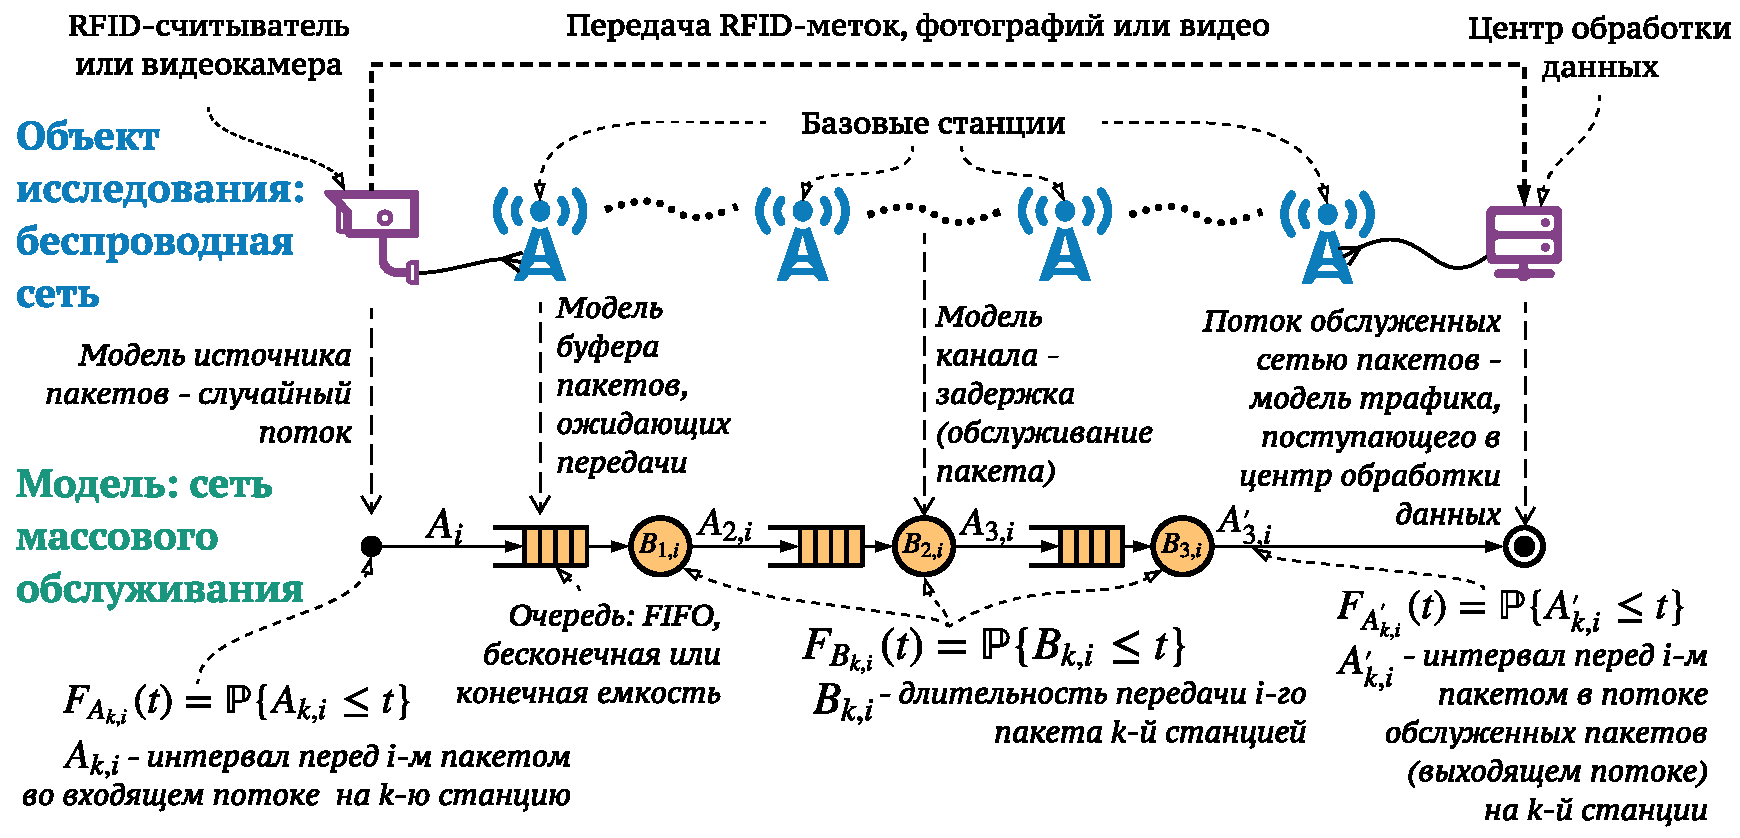
\includegraphics[width=1.0\textwidth]{chapter4/ch4_network_and_model}
  }
  \caption{Беспроводная сеть с линейной топологией и её аналитическая модель.}
  \label{fig:ch4_network_model}
\end{figure}

Для моделирования времени обслуживания будут использоваться PH-распределения $B_i \sim PH(S, \overline{\tau})$, а для моделирования интервалов между поступлениями в сеть пакетов "--- MAP-поток $A \sim MAP(D_0, D_1)$. Определения PH-распределений и MAP-потоков были даны в главе 1, а свойства, необходимые для вычисления характеристик тандемной сети массового обслуживания, будут приведены в следующем разделе.

Поставим формально задачу вычисления средней межконцевой задержки и вероятности потери пакетов из-за переполнения очередей в сети массового обслуживания. Пусть заданы длина сети (число узлов) $N$, емкость очередей $M$, входящий MAP-поток $X \sim MAP(D_0, D_1)$ и PH-распределения времени обслуживания $Y_k \sim PH(S_k, \overline{\tau}_k)$, $k = 1, 2, \dots, N$. Будем обозначать момент поступления $i$-го пакета на вход $k$-го узла как $t_{i,k}^{(a)}$, а момент завершения его обслуживания -- как $t_{i,k}^{(d)}$. Очевидно, что для любого $k < N$ выполняется $t_{i,k}^{(d)} = t_{i,{k+1}}^{(a)}$, если пакет не застает очередь $(k+1)$-го узла заполненной (в этом случае пакет теряется). Рассмотрим произвольный $i$-й пакет. Результатом обработки этого пакета может быть один из двух исходов: либо на некотором $k$-м узле пакет застанет очередь заполненной и будет отброшен, либо он будет обработан последовательно каждым из узлов, и покинет систему тогда, когда завершится его обработка последним узлом в момент $t_{i,N}^{(d)}$. Вероятность первого исхода (то есть потери пакета) будем обозначать $P_l$, она представляет собой долю пакетов, заставших какой-либо узел сети полностью заполненным. Для пакетов, которые не были потеряны, можно вычислить межконцевую задержку $\Delta t_i = t^{(d)}_{i,N} - t^{(a)}_{i,1}$.

Задача исследования состоит в поиске методов численной оценки средней межконцевой задержки $\overline{\Delta t}$ и вероятности потери пакета $P_l$.

Из-за экспоненциального роста размера пространства состояний при увеличении числа станций в сети, вычисление точных значений задержек и вероятностей потери пакетов возможно только для небольших сетей. Для получения оценок параметров в общем случае предлагается использовать метод редукции выходящих потоков, то есть заменять потоки обслуженных пакетов на выходе из очередного узла сети MAP-потоком небольшого размера. Этот метод будет подробно описан и численно исследован в этой главе диссертационной работы.

% На практике обычно известны только статистические оценки распределений или выборка интервалов между пакетами (например, полученная из сетевого дампа). Поэтому при выполнении численных экспериментов в качестве входных данных будем считать известными не сами матрицы $D_0, D_1, S, \overline{\tau}$, а моменты распределений. Пусть $m_a = \mathbb{E}X$ -- среднее время между поступлениями новых пакетов, $\sigma_a$ -- стандартное отклонение. Аналогично, пусть $m_s = \mathbb{E}Y$ -- среднее время обслуживания пакета, а $\sigma_s$ -- его стандартное отклонение. Время обслуживания будем задавать средним значением $m_s$, коэффициентом вариации $c_s = \sigma_s / m_s$ и коэффициентом асимметрии $\gamma_s = \mathbb{E}[(Y - m_s)^3] / \sigma_s^3$. Входящий поток будем задавать аналогично с помощью $m_a$, $c_a$ и $\gamma_a$, а также коэффициента автокорреляции между соседними интервалами $\rho_1$.


%%%%%%%%%%%%%%%%%%%%%%%%%%%%%%%%%%%%%%%%%%%%%%%%%%%%%%%%%%%%%%%%%%%%%%%%%%%%%%%%
\section{Открытая тандемная сеть массового обслуживания с узлами MAP/PH/1/M}\label{sec:ch4_queues}
%%%%%%%%%%%%%%%%%%%%%%%%%%%%%%%%%%%%%%%%%%%%%%%%%%%%%%%%%%%%%%%%%%%%%%%%%%%%%%%%

В этом разделе рассмотрим основные свойства PH-распределений, MAP-потоков и систем массового обслуживания MAP/PH/1/M. На базе этих свойств, сформулируем итерационный алгоритм, позволяющий рассчитывать характеристики сетей массового обслуживания типа MAP/PH/1/M $\rightarrow \bullet$/PH/1/M$\rightarrow \dots \rightarrow \bullet$/PH/1/M, и приведем анализ его сложности.


%%% ~~~~~~~~~~~~~~~~
\subsection{Свойства PH-распределений и MAP-потоков}\label{sec:ch4_queues_map_ph_props}
%%% ~~~~~~~~~~~~~~~~

Пусть $Y \sim PH(S, \overline{\tau})$, матрица $S$ и вектор $\overline{\tau}$ удовлетворяют ограничениям \eqref{eq:ch1_ph_def}. Тогда функция распределения $F(y)$ и моменты случайной величины $Y$ определяются как \cite{Buchholz2014}:

\begin{equation}
	\label{eq:ch4_ph_props}
	\begin{aligned}
		&F(y) = \mathbb{P}\{Y < y\} = 1 - \overline{\tau} e^{Sy} \mathbf{1}\\
		&\mathbb{E}Y^k = k! \overline{\tau} (-S)^{-k} \mathbf{1}
	\end{aligned}
\end{equation}

Пусть $X \sim MAP(D_0, D_1)$, где матрицы $D_0$ и $D_1$ удовлетворяют ограничениям \eqref{eq:ch1_map_def}. Функция распределения интервалов между событиями, значения моментов MAP-потока $X$ и коэффициенты корреляции с лагом $k$ определяются выражениям:

\begin{equation}
	\label{eq:ch4_map_props}
    \begin{aligned}
    \mathbb{P}\{X < t\} &= 1 - \overline{\alpha}e^{D_0 t}\overline{\mathbf{1}}\\
    \mathbb{E}X^{k} &= k! \overline{\alpha}(-D_0)^{-k}\overline{\mathbf{1}}\\
    \rho_k &= \frac{\lambda \overline{\pi} P^k (-D_0)^{-1} \overline{\mathbf{1}} - 1}{2 \overline{\pi} (-D_0)^{-1} \overline{\mathbf{1}} - 1}.
    \end{aligned}
\end{equation}
Матрица $D_1$ описывает переходы управляющей марковской цепи, сопровождающиеся генерацией пакетов (наблюдаемые переходы), а матрица $D_0$ "--- переходы, при которых генерации нового пакета не происходит (невидимые переходы). Если после генерации очередного пакета MAP-поток находится в состоянии $i$, время до появления следующего пакета имеет PH-распределние $X^{(i)} = PH(D_0, \overline{e}_i)$, где $\overline{e}_i = (0, \dots, 0, 1, 0, \dots, 0)$ "--- единичный вектор, в котором на $i$-й позиции стоит единица. Число состояний $W$ в управляющей цепи потока будем называть его размером или порядком и обозначать как $\vline X \vline$.

Стационарное распределение $\overline{\pi} \in \mathbb{R}^W$ вероятностей потока $MAP(D_0, D_1)$ является решением системы линейных уравнений:

\begin{equation}
	\label{eq:ch4_map_pmf}
	\begin{cases}
		\overline{\pi}(D_0 + D_1) &= \overline{\mathbf{0}}\\
		\overline{\pi}\overline{\mathbf{1}} &= 1
	\end{cases},
\end{equation}
где $\overline{\mathbf{0}}$ и $\overline{\mathbf{1}}$ "--- вектор-строки, состоящие из всех нулей и единиц соответственно. Матрица $P = (-D_0)^{-1} D_1$ вложенной цепи и вектор его стационарных вероятностей $\overline{\alpha}$ рассчитываются как:

\begin{equation}
\label{eq:ch4_map_dtmc}
	\overline{\alpha}: \begin{cases}
		\overline{\alpha} P = \overline{\alpha} \\
		\sum\limits_{i=1}^{W} \alpha_i = 1
 	\end{cases}
\end{equation}
Интенсивность MAP-потока можно найти как $\lambda = (\mathbb{E}X)^{-1}$. Её можно вычислить как математическое ожидание случайной величины, равной суммарной интенсивности наблюдаемых переходов:

\begin{equation}
	\label{eq:ch4_map_rate}
	\lambda = \sum\limits_{j=1}^{W} \pi_j \sum\limits_{k=1}^{W} \{D_1\}_{jk} = \overline{\pi} D_1 \overline{\mathbf{1}}
\end{equation}
Формула (\ref{eq:ch4_map_rate})~удобна, когда не требуется вычисление моментов старших порядков или коэффициентов автокорреляции, т.к. в этом случае также не требуется обращать матрицу $D_0$.

\begin{figure}[h]
    \centerfloat{
      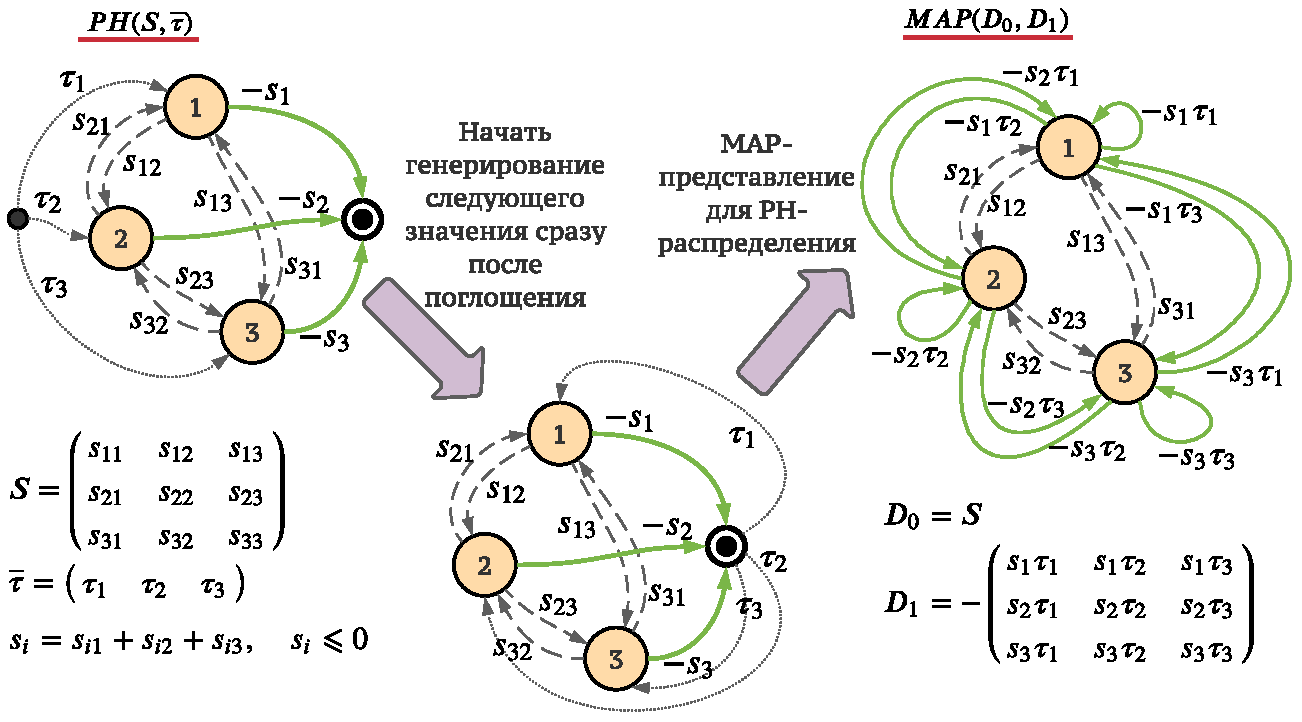
\includegraphics[width=1.0\textwidth]{chapter4/ch4_ph2map}
    }
    \caption{Пример построения MAP-потока, в котором все интервалы имеют одинаковое PH-распределение $PH(S, \overline{\tau})$ с тремя состояниями управляющей цепи.
    \label{fig:ch4_ph2map}}
\end{figure}

MAP-поток является обобщением над PH-распределением. Существенной чертой MAP-потока является то, что корреляция между интервалами может быть отличной от нуля (см. формулу~\eqref{eq:ch4_map_props}). В то же время, последовательность интервалов, каждый из которых имеет PH-распределение с одинаковыми параметрами $PH(S, \overline{\tau})$, также можно считать MAP-потоком, автокорреляция в котором будет нулевой. Для PH-распределения $PH(S, \overline{\tau})$ соответствующий MAP-поток будет иметь матрицы следующего вида:

\begin{equation}
    \label{eq:ch4_map-ph_representation}
    D_0 = S, \qquad D_1 = (-S \overline{1}) \overline{\tau} = -\left(
        \begin{matrix}
            s_1\\
            s_2\\
            \vdots\\
            s_V
        \end{matrix}
     \right) \left(
         \begin{matrix}
            \tau_1 & \tau_2 & \dots &
         \end{matrix}
     \right),
\end{equation}
где $s_i = \sum_{j=1}^V s_{ij}$
Пример построения MAP-потока по PH-распределению приведен на рис.~\ref{fig:ch4_ph2map}.



%%% ~~~~~~~~~~~~~~~~
\subsection{Свойства системы MAP/PH/1/M}\label{sec:ch4_queue_net_system_props}
%%% ~~~~~~~~~~~~~~~~

Ключевое свойство систем массового обслуживания MAP/PH/1/M, благодаря которому их удобно использовать для моделирования многошаговых сетей -- замкнутость на множестве MAP-потоков: согласно следующим теоремам (см. \cite{VishnevskyDudin2018}), результат просеивания MAP-потока "--- MAP-поток, сумма MAP-потоков "--- MAP-поток, и поток обслуженных заявок, выходящих из системы MAP/PH/1/M, также является также MAP-потоком. В дальнейшем будем обозначать выходной поток $Z$ из системы массового обслуживания с входным потоком $X$, временем обслуживания $Y$ и емкостью очереди $M$ как $\mathcal{D}(X, Y, M)$.

\begin{thm}\label{th:ch4_sifted_map}\textnormal{\cite{VishnevskyDudin2018}}
  Результат просеивания MAP-потока $X \sim MAP(D_{0},D_{1})$ с вероятностью $p$ "--- MAP-поток $X_{p} \sim MAP(D_{0}+(1-p)D_{1},pD_{1})$ (в дальнейшем обозначается как $pX$)
\end{thm}

\begin{thm}\label{th:ch4_maps_sum}\textnormal{\cite{VishnevskyDudin2018}}
  Сумма MAP-потоков $X_{1}$ и $X_{2}$, $X_i \sim MAP(D_{0}^{(i)},D_{1}^{(i)})$, $i=1,2$ "--- MAP-поток $X$:
  $$
    X = X_{1} \oplus X_{2} \sim MAP(D_{0}^{(1)} \oplus D_{0}^{(2)},D_{1}^{(1)} \oplus D_{1}^{(2)}),
  $$
  где $\oplus$ "--- сумма Кронекера.
\end{thm}

\textbf{Замечание.} Если потоки $X_1$ и $X_2$ имеют размерности $W_1$ и $W_2$, то размерность суммарного потока $X$ равняется $W = W_1 W_2$.

\begin{thm}\label{th:ch4_map_departure}\textnormal{\cite{VishnevskyDudin2018}}
    Пусть в системе MAP/PH/1/M $X \sim MAP(D_{0}$ $D_{1})$, $D_i \in \mathbb{R}^{W \times W}, i=0,1$ -- входящий поток, $Y \sim PH(S, \overline{\tau})$, $\mathbb{R}^{V \times V}$ -- время обслуживания, обслуживание ведется согласно дисциплине FIFO, а ёмкость очереди равна $M$. Тогда поток выходящих (обслуженных) пакетов есть MAP-поток $Z \sim MAP(D'_{0},D'_{1})$, матрицы которого определяются как:
    \begin{equation}
        \label{eq:ch4_qs_departure_d0}
        D'_{0} =
        \begin{bmatrix}
            D_{0} \otimes I_{V} & D_{1}\otimes (\overline{\tau} \otimes \overline{\mathbf{1}}_{V}) & 0 & \cdots & 0 & 0\\
            0 & D_{0} \otimes S & D_{1} \otimes I_{V} & \cdots & 0 & 0\\
            0 & 0 & D_{0} \otimes S & \cdots & 0 & 0 \\
            \vdots & \vdots & \vdots & \ddots & \vdots & \vdots \\
            0 & 0 & 0 & \cdots & D_{0} \otimes S & D_{1} \otimes I_{V}\\
            0 & 0 & 0 & \cdots & 0 & (D_{0}+D_{1}) \otimes S
        \end{bmatrix},
    \end{equation}
    \begin{equation}
        \label{eq:ch4_qs_departure_d1}
        D'_{1} =
          \begin{bmatrix}
              0 & \cdots & 0 & 0 \\
              I_{W} \otimes C_{t} & \cdots & 0 & 0 \\
              \vdots & \ddots & \vdots & \vdots \\
              0 & \cdots & 0 & I_{W} \otimes C_{t} & 0
          \end{bmatrix},
    \end{equation}
    где $C_{t} = (-S \overline{\mathbf{1}}_{V}) \otimes \overline{\tau}$, а $I_V$, $I_W$ -- едининые матрицы порядка $V$ и $W$ соответственно.
\end{thm}

Из структуры матриц потока $Z$ можно сделать следующие выводы. Во-первых, поток $Z$ имеет размерность $|Z| = (M+2)|X| |Y| = (M+2) V W$. Во-вторых, каждому состоянию потока $Z$ соответствует некоторое число пакетов в системе и состояния входящего MAP-потока $X$ и обслуживающего прибора $Y$. Пусть управляющая цепь потока $Z$ находится в состоянии $n$. Тогда в системе $\lfloor \frac{n}{VW} \rfloor$ пакетов, входящий MAP-поток находится в состоянии $\lfloor \frac{n (\mathbf{mod}\;VW)}{V} \rfloor + 1$, а обслуживающий прибор -- в состоянии $n(\mathbf{mod} V)+1$.

Предыдущее замечание можно обощить. По сути, при построении матриц выходящего MAP-потока производится построение марковской цепи, управляющей работой системы MAP/PH/1/M. Действительно, в такой системе переходы происходят из-за возникновения одного из двух событий: переход в цепи входящего MAP-потока или переход в цепи PH-распределения. При этом, если переход в цепи входящего потока сопровождается формированием сообщения, и система не находится в состоянии полностью заполненной очереди, то размер системы увеличивается. Если же переход происходит в цепи PH-распределения в поглощающее состояние, то размер системы уменьшается на единцицу. Элементы матрицы $D'_0$ соответствуют всем переходам, кроме поглощения в цепи PH-распределения, последним же соответствуют элементы матрицы $D'_1$. По этой причине, когда будет требоваться найти распределение вероятностей управляющей цепи системы MAP/PH/1/M, будем использовать инфинитезимальый генератор управляющей цепи выходящего потока $Z$.

Обозначим $\overline{\pi}$ стационарное распределение $X$, а $\overline{\theta}$ стационарное распределение $Z$. Вектор $\overline{\theta}$ можно переписать в виде $\overline{\theta} = (\overline{\theta}_0, \overline{\theta}_1, \dots, \overline{\theta}_{M+1})$, где $\overline{\theta}_k$ "--- часть вектора $\overline{\theta}$, соответствующая тем состояниям системы, в которых число пакетов равно $k$. Пусть $\mu(t)$ "--- случайный процесс, значение которого в каждый момент времени равняется числу пакетов в системе. Обозначим $p_k = \lim\limits_{t \rightarrow \infty} \mathbb{P}\{\mu(t) = k\}$ "--- стационарная вероятность того, что в системе $k=\overline{0,M+1}$ пакетов. Тогда, зная стационарное распределение $\overline{\theta}$ управляющей цепи MAP-потока $Z$, можно вычислить распределение $\overline{p}$:

\begin{equation}
	\label{eq:ch4_qs_size_pmf}
	p_k = \sum\limits_{j=1}^{VW} \{ \overline{\theta}_k \}_j.
\end{equation}
Отсюда можно рассчитать среднее число пакетов в системе как $m_1 = \mathbb{E}\mu$:

\begin{equation}
  \label{eq:ch4_qs_size_avg}
  \begin{aligned}
	  m_1 = \sum\limits_{k=0}^{M+1} k \mathbb{P}\{\mu = k\} = \sum\limits_{k=0}^{M+1} k p_k = \sum\limits_{k=0}^{M+1} k \sum\limits_{j=1}^{VW} \{ \overline{\theta}_k \}_j = \sum\limits_{k=0}^{M+1} \sum\limits_{j=1}^{VW} k \theta_{kVW+j}\hfill.
  \end{aligned}
\end{equation}

Для получения вероятности потери пакета из-за переполнения очереди нужно более подробно рассмотреть часть вектора $\overline{\theta}$, соответствующую случаю заполненной очереди (т.е. $\mu=M+1$). Состояния внутри блоков матриц \eqref{eq:ch4_qs_departure_d0} и \eqref{eq:ch4_qs_departure_d1} сгруппированы по состояниям входящего MAP-потока, т.е. состояния $\{ \overline{\theta}_k \}_{jV + 1}, \dots \{ \overline{\theta}_k \}_{(j+1)V}$ соответствуют всевозможным состояниям цепи PH-распределения и состоянию $j$ входящего MAP-потока, когда в системе $k$ пакетов. Определим:

\begin{equation}
    \label{eq:ch4_qs_size_slice_pmf}
    \overline{\psi}_k = ( \sum\limits_{j=1}^{V}\{ \overline{\theta}_k \}_j, \dots, \sum\limits_{j=1}^{V}\{ \overline{\theta}_{k} \}_{(W-1)V + j} )
\end{equation}
"--- распределение вероятностей входящего MAP-потока при $k$ пакетах в системе. Тогда вероятность $P_L$ потери пакета можно выразить так:

\begin{equation}
  \label{eq:ch4_qs_loss_prob}
  P_L = \overline{\psi}_{M+1} \frac{D_1}{\lambda_X}\overline{\mathbf{1}}
\end{equation}

Наконец, зная интенсивность входящего потока $\lambda_{X}$, среднее число пакетов в системе $m_1$ и вероятность потери пакетов $P_L$, используя формулу Литтла, можно рассчитать среднюю задержку:

\begin{equation}
	\label{eq:ch4_qs_delay}
	T = \frac{m_1}{(1 - P_L)\lambda_{X}}.
\end{equation}
Множитель $(1 - P_L)$ в знаменателе возникает в следствие того, что из-за переполнения очереди лишь часть пакетов входящего потока попадает в систему, т.е. фактическая интенсивность потока пакетов, поступающих в систему, составляет $(1 - P_L) \lambda_{X}$.



%%% ~~~~~~~~~~~~~~~~
\subsection{Точный расчёт характеристик сети массового обслуживания}\label{sec:ch4_queue_net_precise}
%%% ~~~~~~~~~~~~~~~~


Используя формулы \eqref{eq:ch4_qs_size_avg}, \eqref{eq:ch4_qs_loss_prob} и \eqref{eq:ch4_qs_delay} несложно вычислить среднюю межконцевую задержку пакетов в сети и вероятность потери пакета на каком либо узле. Будем рассматривать два варианта сетей: сети с кросс-трафиком, в которых потоки данных поступают на каждый узел, и сети без кросс-трафика, в которых внешний трафик поступает только на первую станцию, и все последующие станции передают только его.

\begin{figure}[htb]
	\centerfloat{
    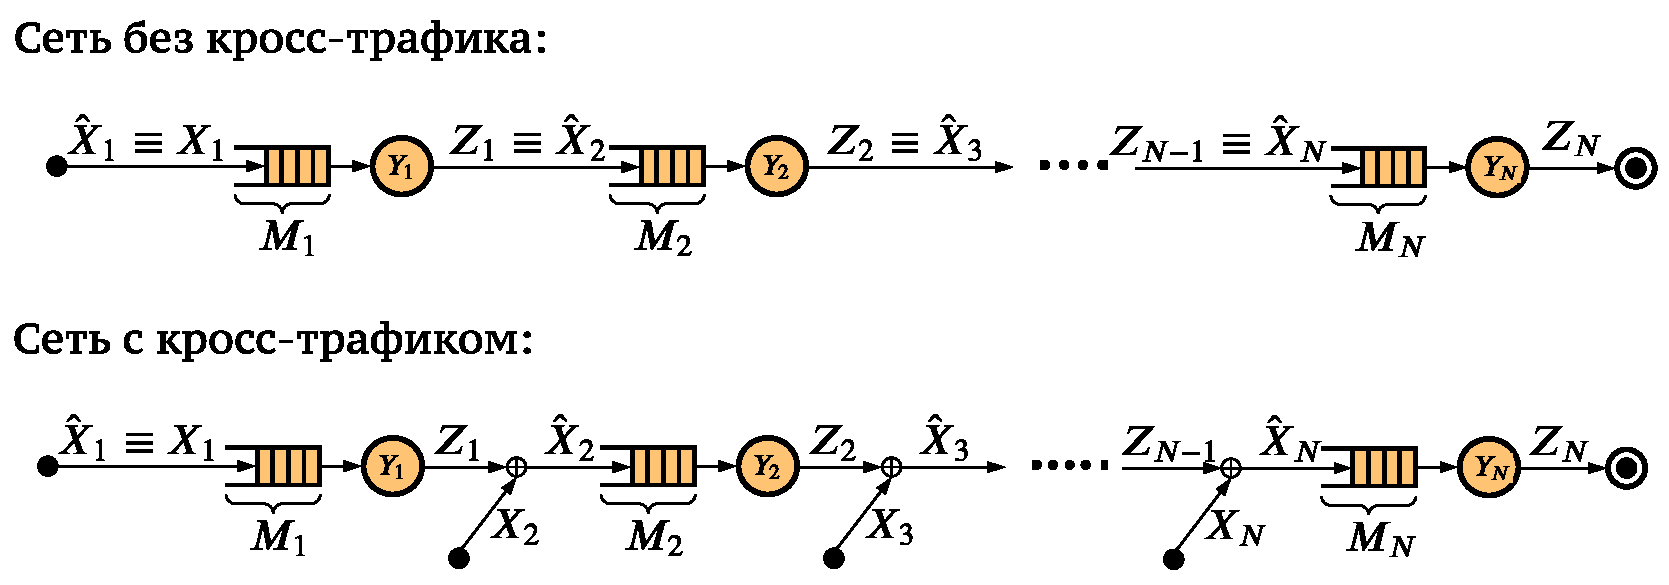
\includegraphics[width=1.0\textwidth]{chapter4/ch4_queueing_networks}
  }
  \caption{Сети массового обслуживания с кросс-трафиком и без него.}
  \label{fig:ch4_queueing_networks}
\end{figure}

Пусть в сети (см. рис. \ref{fig:ch4_queueing_networks}) $N$ станций, емкость очереди на $i$-й станции ($i = 1,2, \dots, N$) равна $M_i \in \mathbb{N}$, а длительность обслуживания $Y_i$ имеет PH-распределение $Y_i \sim PH(S_i, \overline{\tau})$, $S_i \in \mathbb{R}^{V_i \times V_i}$, $V_i \in \mathbb{N}$. Если в сети есть кросс-трафик, то на каждую станцию поступает пользовательский поток $X_i \sim MAP(D_{0,i}, D_{1,i})$; если кросс-трафика нет, то поток $X_1 \equiv X = MAP(D_0, D_1)$ поступает только на первую станцию. Обозначим порядок входящего MAP-потока на $i$-ю станцию как $W_i$, то есть $D_{0,i}, D_{1,i} \in \mathbb{R}^{W_i \times W_i}$, $W_i \in \mathbb{N}$.

Обозначим $Z_i$ - выходящий MAP-поток с $i$-й станции, а $\hat{X}_i$ - общий входящий поток на $i$-ю станцию. Тогда, согласно теоремам \ref{th:ch4_maps_sum} и \ref{th:ch4_map_departure}, потоки $\hat{X}_i$ и $Z_i$ "--- MAP-потоки. Используя ранее введённые обозначения, их можно определить формально следующим образом:

\begin{equation}
  \label{eq:ch4_total_arrival_and_departure}
  \begin{aligned}
    \hat{X}_1 &\equiv X_1\\
    \hat{X}_i &= \begin{cases}
      X_i \oplus Z_{i-1},&\text{в сети есть кросс-трафик и } i = 2,3, \dots, N\\
      Z_{i-1},&\text{в сети нет кросс-трафика}
    \end{cases}\\
    Z_i &= \mathcal{D}(\hat{X}_i, Y_i, M)
  \end{aligned}
\end{equation}

Обозначим порядок выходящих MAP-потоков $Z_i$ как $U_i$, $i=1,2,\dots N$, то есть $Z_i \sim MAP(\tilde{D}_{i,0}, \tilde{D}_{i,1})$ и $\tilde{D}_{i,0}, \tilde{D}_{i,1} \in \mathbb{R}^{U_i \times U_i}$. Тогда величина $U_i$ определяется с помощью следующего утверждения.

\begin{prop}\label{prop:ch4_departure_order}
	Порядок $U_i$ MAP-потока обслуженных пакетов $Z_i$ на выходе из $i$-го узла, $i = 1,2,\dots N$, определяется как:
	$$
	U_i = \begin{cases}
		\prod\limits_{j=1}^{i}(M_j + 2)V_jW_j,&\text{если в сети есть кросс-трафик}\\
		W_1\prod\limits_{j=1}^{i}(M_j + 2)V_j,&\text{если кросс-трафика нет}.
	\end{cases}
	$$
\end{prop}
\begin{proof}
Утверждение доказывается по индукции. При $i = 1$ $Z_1 = \mathcal{D}(X_1, Y_1, M_1)$ и $U_1 = (M_1 + 2)V_1W_1$ согласно замечанию к теореме \ref{th:ch4_map_departure}.

Пусть утверждение верно при $i = n-1$. Если в сети нет кросс-трафика, то $Z_i = \mathcal{D}(\hat{X}_i, Y_i, M_i) = \mathcal{D}(Z_{i-1}, Y_i, M_i)$ и величина $U_i$ определяется как:
$$
  \begin{aligned}
    U_i &= (M_i + 2) V_i U_{i-1} = (M_i + 2) V_i \times (W_1 \prod\limits_{j=1}^{i-1}(M_j + 2)V_j)\\
    &= W_1 \prod\limits_{j=1}^{i}(M_j + 2)V_j.
  \end{aligned}
$$
Если же в сети есть кросс-трафик, то
$$
  Z_i = \mathcal{D}(\hat{X}_i, Y_i, M_i) = \mathcal{D}(Z_{i-1} \oplus X_i, Y_i, M_i),
$$
и порядок потока $Z_i$ определяется следующей цепочкой равенств:
$$
  \begin{aligned}
    U_i &= (M_i + 2) V_i (U_{i-1} W_i) = (M_i + 2) V_i W_i \times \prod\limits_{j=1}^{i-1}(M_j + 2) V_j W_j)\\
    &= \prod\limits_{j=1}^{i}(M_j + 2) V_j W_j.
  \end{aligned}
$$
\end{proof}

Схема расчёта характеристик сети выглядит следующим образом.

\textit{Шаг 1.} Положим $i := 1$.

\textit{Шаг 2.} Если $i = 1$, то положим $\hat{X}_i = X_1$. Если же $i > 1$, то вычисляем $\hat{X}_i$ согласно \eqref{eq:ch4_total_arrival_and_departure}: $\hat{X}_i = Z_{i-1}$, если в сети нет кросс-трафика, и $\hat{X}_i = Z_{i-1} \oplus X_i$ иначе. Обозначим матрицы потока $\hat{X}_i$ как $\hat{D}_{i,0}$ и $\hat{D}_{i,1}$, то есть $\hat{X}_i = MAP(\hat{D}_{i,0}, \hat{D}_{i,1})$.

\textit{Шаг 3.} С помощью теоремы \ref{th:ch4_map_departure} вычисляем матрицы $D'_{i,0}$, $D'_{i,1}$ MAP-потока $Z_i = \mathcal{D}(\hat{X}_i, Y_i, M_i)$.

\textit{Шаг 4.} Для выходящего MAP-потока $Z_i$ вычисляем его стационарное распределение $\overline{\theta}^{(i)}$ с помощью системы линейных алгебраических уравнений:
$$
  \begin{cases}
	  \overline{\theta}^{(i)}(D'_{i,0} + D'_{i,1}) &= 0\\
	  \overline{\theta}^{(i)} \mathbf{1} &= 1
  \end{cases}
$$

\textit{Шаг 5.} Рассчитываем среднее число пакетов в очереди $i$-й станции согласно \eqref{eq:ch4_qs_size_avg}:
$$
  m_1^{(i)} = \sum\limits_{k=0}^{M_i + 1} k \sum\limits_{j=1}^{V_i \hat{W}_i} \theta^{(i)}_{k V_i \hat{W}_i + j}\;,
$$
где $V_i = |Y_i|$ "--- порядок PH-распределения $Y_i$, а $\hat{W}_i = |\hat{X}_i|$ "--- порядок входящего MAP-потока $\hat{X}_i$.

\textit{Шаг 6.} Определяем стационарное распределение вероятностей $\overline{\pi}^{(i)}$ входящего потока $\hat{X}_i$. Если в сети нет кросс-трафика и $i > 1$, то полагаем $\overline{\pi}^{(i)} \equiv \overline{\theta}^{(i-1)}$. В противном случае находим $\overline{\pi}^{(i)}$ как решение системы линейных алгебраических уравнений:
$$
  \begin{cases}
	  \overline{\pi}^{(i)}(\hat{D}_{i,0} + \hat{D}_{i,1}) &= 0\\
	  \overline{\pi}^{(i)} \mathbf{1} &= 1
  \end{cases}
$$

\textit{Шаг 7.} С помощью найденного на предыдущем шаге стационарного распределения $\overline{\pi}^{(i)}$ входящего потока $\hat{X}_i$ и формулы \eqref{eq:ch4_map_rate} вычисляем интенсивность поступления пакетов на $i$-ю станцию:
$$
  \lambda_i = \overline{\pi}^{(i)} \hat{D}_{i,1} \overline{\mathbf{1}}.
$$

\textit{Шаг 8.} Рассчитываем распределение состояний входящего MAP-потока при наличии в системе $M_i + 1$ пакета (то есть при заполненной системе):
$$
  \overline{\psi}^{(i)} = \left(
  \sum\limits_{j=1}^{V_i} \{ \overline{\theta}^{(i)}_{M_i+1} \}_j,
  \dots,
  \sum\limits_{j=1}^{V_i} \{ \overline{\theta}^{(i)}_{M_i+1} \}_{(\hat{W}_i-1) V_i + j}
  \right).
$$
Здесь вектор $\overline{\theta}_{M_i+1}^{(i)}$ "--- часть вектора $\overline{\theta}^{(i)}$, относящаяся к состояниям системы, когда в ней находится $M_i + 1$ пакет.

\textit{Шаг 9.} Вычисляем векроятность потери пакета из-за переполнения $i$-й очереди с помощью~\eqref{eq:ch4_qs_loss_prob}:
$$
  P_L^{(i)} = \overline{\psi}^{(i)} \frac{\hat{D}_{i,0}}{\lambda_i} \overline{\mathbf{1}}.
$$

\textit{Шаг 10.} Вычисляем среднюю задержку пакетов на $i$-й станции с помощью~\eqref{eq:ch4_qs_delay}:
$$
  T_i = \frac{m_1^{(i)}}{(1 - P_L^{(i)}) \lambda_i}
$$

\textit{Шаг 11.} Если $i < N$, то увеличиваем $i := i + 1$ и переходим на шаг 2. В противном случае переходим далее, на шаг 12.

\textit{Шаг 12.} Вычисляем вероятность потери пакета $P_L = \prod\limits_{i=1}^{N} (1 - P_L^{(i)})$.

\textit{Шаг 13.} Вычисляем общую задержку $T = \sum\limits_{i=1}^{N} T_i$.

Предложенная схема проста в вычислении. По сути, на каждом шаге с помощью нескольких операций произведения Кронекера строятся блочные матрицы для выходящего MAP-потока, а также, если в сети есть кросс-трафик, с помощью суммы Кронекера строятся матрицы входящего потока. Далее решаются две (если в сети есть кросс-трафик) или одна (в противном случае) системы линейных алгебраических уравнений для определения стационарных вероятностей входящего и исходящего потока. Наконец, с помощью нескольких операций умножений найденных распределений на матрицы потоков, вычисляются искомые характеристики "--- вероятность потери пакета, средний размер системы и задержка.

Главный недостаток этой схемы расчета "--- чрезвычайно высокая вычислительная сложность.

\begin{prop}\label{prop:ch4_base_algorithm_complexity}
  Пусть входящие MAP-потоки имеют порядок $W$, PH-распределения "--- порядок $V$, ёмкость очередей равна $M$, и сеть содержит $N$ станций. Тогда итерационная схема расчета характеристик тандемной сети имеет сложность:
  \begin{itemize}
	  \item $O((M V W)^{3N})$, если в сети есть кросс-трафик
	  \item $O(W^3 (M V)^{3N})$, если кросс-тррафика в сети нет.
  \end{itemize}
\end{prop}
\begin{proof}
Рассмотрим $i$-ю итерацию алгоритма, $i \leqslant N$, то есть расчёт характеристик $i$-й станции сети. Отметим сперва, что при $i > 1$ порядок выходящего потока с предыдущей $i-1$-й станции есть $(M + 2) V \hat{W}_i$, где $\hat{W}_i$ "--- порядок входящего потока на $i$-ю станцию. Согласно \ref{prop:ch4_departure_order}, при наличии в сети кросс трафика $U_i = ((M+2)VW)^i$, а если кросс-трафика нет, то $U_i = W((M+2)V)^i$.

Сложность итерации определяется шагами 4 и 6, в которых необходимо решать системы линейных алгебраических уравнений, причем порядок матрицы системы на шаге 4 (генератор выходящего потока) заведомо выше, чем системы на шаге 6 (генератор входящего потока). Полагая, что для решения системы используется алгоритм наподобии метода Гаусса, на шаге 4 потребуется $O(U_i^3)$ операций. Остальные шаги имеют более низкую сложность: шаги 1, 10 и 11 "--- $O(1)$, шаг 2 "--- $O(U_{i-1}^2 W^2)$, шаг 3 "--- $O(U_i^2)$, шаг 5 "--- $O(VW + M)$, шаги 7 и 9 "--- $O(U_i^2)$, шаг 8 "--- $O(VM)$. Сложность шагов 12 и 13 есть $O(N)$.

Таким образом, если в сети есть кросс-трафик, сложность алгоритма составит
$$
  \begin{aligned}
    O((VWM)^3) &+ O((VWM)^6) + \dots + O((VWM)^{3N}) + O(N) \\
    &= O(VWM)^{3N},
  \end{aligned}
$$
а если кросс-трафика в сети нет, то
$$
  \begin{aligned}
    O(W^3 (VM)^3) &+ O(W^3 (VM)^6) + \dots + O(W^3 (VM)^{3N}) + O(N) \\
    &= O(W^3 (VM)^{3N}).
  \end{aligned}
$$

\end{proof}

\textbf{Замечание 1.} Учитывая, что матрицы выходящего потока $Z_i$ имеют блочный трехдиагональный вид, они будут сильно разрежены. Благодаря этому можно попытаться применить более эффективные способы решения системы алгебраических уравнений. Однако, показатель степени в оценке сложности все равно не окажется ниже, чем $(2 + \epsilon) N$.


На практике утверждения \ref{prop:ch4_departure_order} и \ref{prop:ch4_base_algorithm_complexity} означают, что искать решения с помощью представленной схемы вычислений становится невозможным даже при относительно небольших $N$, $V$ и $W$. В таблице \ref{table:ch4_map_order_growth} приведены примеры роста порядков для различных порядков входящих процессов и времен обслуживания.

\begin{table}[h!]
\centering
\begin{tabular}{ |c|c|c||c|c|c|c|c| }
\hline
\multicolumn{3}{|c||}{} & \multicolumn{5}{c|}{Номер станции} \\
\hline
%\multirow{2}{4em}{Сеть без кросс-трафика, число станций}\\
$W$ & $V$ & $M$ & 1 & 2 & 3 & 4 & 5\\
\hline
\multicolumn{8}{|c|}{Сети без кросс-трафика} \\
\hline
1 & 1 & 1 & 3 & 9 & 27 & 81 & 243 \\
1 & 1 & 3 & 5 & 25 & 125 & 625 & 3'125 \\
2 & 2 & 2 & 16 & 128 & 1'024 & 8'192 & 65'536 \\
3 & 1 & 3 & 15 & 75 & 375 & 1'875 & 9'375 \\
1 & 3 & 3 & 15 & 225 & 3'375 & 50'625 & 759'375 \\
3 & 3 & 3 & 45 & 675 & 10'125 & 151'875 & 2'278'125 \\
\hline
\multicolumn{8}{|c|}{Сети с кросс-трафиком} \\
\hline
1 & 1 & 1 & 3 & 9 & 27 & 81 & 243 \\
1 & 1 & 3 & 5 & 25 & 125 & 625 & 3'125 \\
2 & 2 & 2 & 16 & 256 & 4'096 & 65'536 & 1'048'576 \\
3 & 1 & 3 & 15 & 225 & 3'375 & 50'625 & 759'375 \\
1 & 3 & 3 & 15 & 225 & 3'375 & 50'625 & 759'375 \\
3 & 3 & 3 & 45 & 2'025 & 91'125 & 4'100'625 & 184'528'125 \\
\hline
\end{tabular}
\caption{Порядки выходящих MAP-потоков в зависимости от порядков PH-распределения ($V$), входящих MAP-потоков ($W$) и ёмкости очереди ($M$).\label{table:ch4_map_order_growth}
}
\end{table}

Таким образом, для практического применения открытых сетей с узлами MAP/PH/1/M необходимы более эффективные методы расчета, пусть даже их результаты будут приближенными.




%%%%%%%%%%%%%%%%%%%%%%%%%%%%%%%%%%%%%%%%%%%%%%%%%%%%%%%%%%%%%%%%%%%%%%%%%%%%%%%%
\section{Расчёт характеристик сети массового обслуживания методом Монте-Карло}
%%%%%%%%%%%%%%%%%%%%%%%%%%%%%%%%%%%%%%%%%%%%%%%%%%%%%%%%%%%%%%%%%%%%%%%%%%%%%%%%

Расчёт методом Монте-Карло заключается в многократном проигрывании прохождения пакетов по сети массового обслуживания и замерах длительностей их пребывания в узлах, длин очередей и потерь. Для реализации этого метода лучше всего подходят системы дискретно-событийного моделирования, в которых обрабатываются возникающие события, а время изменяется только в начале обработки очередного события.

Методы и алгоритмы имитационного моделирования открытых сетей массового обслуживания хорошо известны, поэтому далее приведем лишь краткое схематичное описание работы модели и способа расчёта характеристик сети.

Для моделирования сети с узлами MAP/PH/1/M нужно описать обработку двух типов событий: появление нового пакета во входящем MAP-потоке и завершение обработки пакета на узле.

Пусть, как и ранее, $N$ "--- число станций в сети. Обозначим $K$ "--- глобальный счетчик пакетов, $T_k^a$ "--- время появления $k$-го пакета, $\Delta$ "--- множество вычисленных задержек, $a_i$ "--- число сгенерированных пакетов из $i$-го потока, $l_i$ "--- число потерянных пакетов на $i$-й станции, $t$ "--- модельное время, $n_i$ "--- число пакетов на $i$-й станции.

Если какая-либо из перечисленных величин $\chi$ будет нас интересовать в определенный момент модельного времени $t$, то будем писать $\chi(t)$. Кроме того, при описании операций будем использовать запись $\chi' := f(\chi)$, подразумевая, что после завершения выполнения текущего действия величина $\chi$ примет значение $\chi'$, а до окончания операции она сохраняет значение $\chi$.


%%% ~~~~~~~~~~~~~~~~
\subsection{Обработка событий}
%%% ~~~~~~~~~~~~~~~~

При \textbf{инициализации} модели для каждого потока $X_i$ выбирается интервал до поступления первого пакета $\tau_i$, и на время $\tau_i$ назначается обработка события поступления пакета на $i$-ю станцию.

Рассмотрим действия, происходящие при возникновении событий поступления нового пакета и завершении обслуживания.

\textbf{Обработка поступления нового пакета.} Если в момент времени $t = t_0$ во входящем потоке, поступающем в узел с номером $i$, происходит появление пакета, выполняются следующие действия.

\textit{Шаг 1.} Пакет обрабатывается в зависимости от того, занят ли прибор и есть ли место в очереди:
\begin{itemize}
  \item Если $n_i = 0$, то есть обслуживающий прибор узла $i$ свободен, то вычисляется случайная длительность обслуживания $\tau_s$, $\mathbb{P}\{\tau_s \leqslant \tau\} = F_{Y_i}(\tau)$, на момент времени $t_0 + \tau_s$ назначается событие окончания обслуживания на $i$-м приборе, а число пакетов в системе увличивается на единицу: $n'_i := n_i + 1$.
  \item Если $1 \leqslant n_i \leqslant M_i$, то есть обслуживающий прибор занят, но в очереди есть место, то пакет помещается в очередь, и счётчик числа пакетов в системе увличивается на единицу: $n'_i := n_i + 1$.
  \item Если $n_i = M_i + 1$, то есть в очереди нет места, пакет теряется, а счётчик потерянных пакетов $l_i$ увеличивается на единицу: $l'_i := l_i + 1$.
\end{itemize}

\textit{Шаг 2.} Для пакета сохраняется время его появления $T_K^a := t_0$.
\textit{Шаг 3.} Счётчики числа сгенерированных пакетов $K$ и $a_i$ увеличиваются на единицу: $K' := K + 1$, $a'_i := a_i + 1$.
\textit{Шаг 4.} Выбирается случайное время до следующего появления пакета в $i$-м потоке $\tau_a$, $\mathbb{P}\{ \tau_a \leqslant \tau \} = F_{X_i}(\tau)$, на момент $t_0 + \tau_a$ назначается следующее событие появления нового пакета в $i$-м потоке.

\textbf{Завершение обслуживания пакета.} Если в момент времени $t_0$ завершается обслуживание $k$-го пакета в узле $i$, то выполняется следующее:

\textit{Шаг 1.} Если $i < N$, то пакет обрабатывается в зависимости от того, занят ли прибор на следующей станции, и есть ли место в её очереди:
\begin{itemize}
\item Если $n_{i+1} = 0$, то есть обслуживающий прибор узла $i+1$ свободен, то вычисляется случайная длительность обслуживания $\tau_s$, $\mathbb{P}\{\tau_s \leqslant \tau\} = F_{Y_{i+1}}(\tau)$, на момент времени $t_0 + \tau_s$ назначается событие окончания обслуживания на $i+1$-м приборе, а число пакетов в системе увеличивается на единицу: $n'_{i+1} := n_{i+1} + 1$.
\item Если $1 \leqslant n_{i+1} \leqslant M_{i+1}$, то есть обслуживающий прибор занят, но в очереди есть место, то пакет помещается в очередь $i+1$-й станции и увеличивается счётчик числа пакетов в системе: $n'_{i+1} := n_{i+1} + 1$.
\item Если $n_{i+1} = M_{i+1}$, то есть в очереди нет места, то пакет теряется, а счётчик потерянных пакетов $l_{i+1}$ увеличивается на единицу: $l'_{i+1} := l_{i+1} + 1$.
\end{itemize}

\textit{Шаг 2.} Если $i = N$, то в $\Delta$ добавляется величина $t_0 - T_k^a$, то есть время с появления пакета до натоящего времени.
\textit{Шаг 3.} Число пакетов на $i$-й станции уменьшается: $n'_i := n_i - 1$.
\textit{Шаг 4.} Если в очереди $i$-й станции есть еще пакеты, то есть $n_i > 0$, то вычисляется случайная длительность обслуживания $\tau_s$, $\mathbb{P}\{\tau_s \leqslant \tau\} = F_{Y_i}(\tau)$, на момент времени $t_0 + \tau_s$ назначается событие окончания обслуживания на $i$-м приборе.



%%% ~~~~~~~~~~~~~~~~
\subsection{Расчет характеристик}
%%% ~~~~~~~~~~~~~~~~

В момент времени $t$ межконцевую среднюю задержку $\overline{T}(t)$ можно оценить как
$$
\overline{T}(t) = \frac{1}{|\Delta(t)|}\sum\limits_{\delta \in \Delta(t)} \delta,
$$
а вероятность успешной доставки пакета $P_s(t)$ "--- как долю доставленных пакетов из всех пакетов, успевших к моменту времени $t$ покинуть систему.
$$
P_s(t) = 1 - \frac{\sum\limits_{i=1}^{N} l_i(t)}{K(t) - \sum\limits_{i=1}^{N} n_i}
$$

Симуляция производится либо до достижения модельным временем заданного значения $T_{max}$, либо до того, как отклонение искомых характеристик не становится меньше заданной величины $\epsilon$. Для реализации последнего критерия, можно вычислять оценки $\overline{T}(t)$ и $P_s(t)$ в моменты модельного времени $t_1, t_2, \dots$ и останавливать симуляцию в момент времени $t_n$, если $\left(\overline{T}(t_n) - \overline{T}(t_{n-1}) \right) / \overline{T}(t_n) < \epsilon$ и $\left( P_s(t_n) - P_s(t_{n-1}) \right) / P_s(t_{n-1}) < \epsilon$.

Для повышения достоверности результатов можно провести симуляцию несколько раз, и в качестве результатов эксперимента использовать усреднённые значения по всем проведённым симуляциям.



%%% ~~~~~~~~~~~~~~~~
\subsection{Программная реализация}
%%% ~~~~~~~~~~~~~~~~

Выбор конкретных алгоритмов и методов реализации имитационной модели зависит от того, используется ли готовая система имитационного моделирования, или же модель пишется без использования готовых систем. Рпакеты для моделирования систем массового обслуживания входят в известные такие системы, как OMNeT++, MatLab, AnyLogic и другие.

В диссертационном исследовании автором была разработана высокоэффективная реализацию модели сети с MAP-потоками и PH-распределениями на языке C++, и разработан интерфейс для ее подключения в код на Python с помощью Cython. Реализация доступна в пакете \texttt{pyqumo} на GitHub: \url{https://github.com/ipu69/pyqumo}. Все алгоритмы для расчета характеристик в имитационной модели реализованы так, чтобы использовать ограниченный объем памяти. Кроме реализации имитационной модели, пакет содержит классы для представления MAP-потоков, PH-распределений, систем MAP/PH/1/M и методы для аналитического расчета их характеристик.


%%% ~~~~~~~~~~~~~~~~
\subsection{Преимущества и недостатки метода}
%%% ~~~~~~~~~~~~~~~~
Главное преимущество метода Монте-Карло для вычисления характеристик сети массового обслуживания "--- его простота. Так как при выполнении модели не происходит явного построения выходных потоков, нет и экспоненциального роста размера задачи при увеличении числа станций. Точность получаемых результатов связана только со временем, которое выделено для проведения эксперимента. Наконец, в реальной имитационной модели собирается гораздо больше характеристик сети, чем было описано выше. Например, вычисляются оценки моментов и коэффициентов автокорреляции в выходных потоках и средние длины очередей.

Метод также обладает серьезными недостатками, основной из которых "--- невозможность эффективного повторного использования результатов: даже при небольшом изменении входных данных (например, размера сети или одного из входных потоков) требуется заново выполнять весь эксперимент. Если MAP-потоки или PH-распределения имеют большие размерности, для генерации случайных величин нужно больше времени. Также много времени требуется, если сеть содержит большое число станций.

Главный недостаток метода Монте-Карло "--- зависимость точности результатов от числа промоделированных событий. Это означает, что какой бы эффективной не была реализация, для получения качественных результатов все равно потребуется сгенерировать определенное число случайных величин. Например, при моделировании сети с десятью узлами для получения высокой точности с погрешностью в пределах 5\% приходится генерировать порядка 100000 пакетов. Таким образом, у метода Монте-Карло оказывается весьма ограниченный потенциал к ускорению вычислений. Так, можно ускорить вычисление с нескольких секунд до ста милисекунд, за счет использования более эффективных алгоритмов обработки статистики, более быстрых структур данных и других оптимизаций, но нельзя получить время, меньшее, чем требуется для генерации $N$ экспоненциально-распределенных случайных величин, причем это число $N$ может иметь порядок $10^5-10^7$. Как будет показано далее, в ходе численного эксперимента было обнаружено, что использование аппроксимаций выходящих потоков позволяет получить результаты в среднем даже быстрее, хотя и с несколько меньшей точностью.

Для получения оценок исследуемых характеристик за существенно меньшее время (порядка микросекунд) нужно использовать радикально иной подход, позволяющий отказаться от необходимости генерировать большое число случайных величин. В качестве такого подхода можно использовать, например, машинное обучение. Подробное рассмотрение данного метода выходит за рамки диссертационной работы.


%%% ~~~~~~~~~~~~~~~~
\section{Расчёт характеристик сети методом понижения размерности выходящих потоков}
%%% ~~~~~~~~~~~~~~~~

В качестве альтернативы методу Монте-Карло, для расчёта характеристик открытой сети массового обслуживания с узлами MAP/PH/1/M в настоящей работе предлагается использовать метод итерационного расчёта с понижением размерности выходящих потоков. Идея метода заключается в том, чтобы заменять MAP-потоки обслуженных пакетов другими MAP-потоками, имеющими те же или близкие значения первых $K$ моментов и коэффициентов автокорреляции с лагами $1, 2, \dots L$, но порядок которых ограничен заданной константой $W$. В этом случае экспоненциального роста размерности исходящих потоков нет: исходящий поток из любой станции имеет порядок не выше $(M_i + 2) V_i (W + W_i)$, где $M_i$ "--- ёмкость очереди на $i$-й станции, $V_i$ "--- порядок PH-распределения $i$-го обслуживающего прибора, $W_i$ "--- порядок внешнего MAP-потока, поступающего на $i$-ю фазу. Если кросс-трафика нет и $i > 1$, то в этой форумле $W_i = 0$, а если $i = 1$, то $W = 0$.

Основная сложность, связанная с применением метода понижения размерностей заключается в том, что даже по известным значениям моментов и коэффициентов автокорреляции сложно сделать вывод о том, какова минимальная размерность MAP-потока, имеющего такие характеристики. По этой причине, вместо поиска MAP-потока, имеющего точно заданные моменты и коэффициенты автокорреляции, будем искать MAP-поток, имеющий достаточно близкие значения этих характеристик.

Будем использовать три различных подхода к построению аппроксимирующих MAP-потоков:

\begin{enumerate}
\item Обобщенный метод моментов.
\item Метод независимого приближения моментов и коэффициента автокорреляции первого порядка, описанный в работе Horvath \cite{Horvath2005}.
\item EM-алгоритм, описанный в работах Horvath, Okamura и Dohi \cite{Okamura2009,Horvath2013}.
\end{enumerate}

Построения MAP-потока методом моментов сводится к поиску решения задачи нелинейного программирования, для постановки которой нужно знать только значения моментов и коэффициентов автокорреляции. Эти величины могут быть вычислены по известным матрицам потока $Z_i$ с помощью формул \eqref{eq:ch4_map_moments} и \eqref{eq:ch4_map_lag_k}. В отличие от метода моментов, для работы EM-процедуры нужна выборка значений интервалов из аппроксимируемого MAP-потока, поэтому для её работы нужно сгенерировать выборку достаточного размера из MAP-потока $Z_i$. Для использования метода независимого приближения моментов и коэффициента автокорреляции первого порядка можно использовать как выборку, так и значения моментов.

Если для работы алгоритма восстановления MAP-потока $\mathcal{A}_o$ нужны $K_m$ первых моментов и $K_l$ первых коэффициентов автокорреляции, то шаг 2 схемы расчёта, описанной в разделе \ref{sec:ch4_iterative_procedure} заменяется шагом $2^*$:

\textit{Шаг $2^*$}. Если $i = 1$, то положим $\hat{X}_i = X_1$. В противном случае ($i > 1$):
\begin{enumerate}
\item Для потока $Z_{i-1} \sim MAP(\tilde{D}_0, \tilde{D}_1)$ вычисляем $P$ и $\overline\alpha$ согласно \eqref{eq:ch4_map_embedded_process}.
\item Вычисляем $\overline\mu \in \mathbb{R}^{K_m}$, $\mu_i = i! \overline\alpha (-\tilde{D}_0)^{-i} \overline{\mathbf{1}}$
\item Вычисляем $\overline\nu \in \mathbb{R}^{K_l}$, $\nu_i = \frac{\overline\theta P^i (-\tilde{D}_0)^{-1} \overline{\mathbf{1}} - 1}{\mu_1 \left( 2 \overline\theta (-\tilde{D}_0)^{-1} \overline{\mathbf{1}} - 1 \right)}$.
\item Находим $Z'_{i-1} = \mathcal{A}_o(\overline\mu, \overline\nu)$
\item Если в сети есть кросс-трафик, то полагаем $\hat{X}_i = Z'_{i-1} \oplus X_i$, а в противном случае $\hat{X}_i = Z'_{i-1}$.
\end{enumerate}
При расчёта коэффициентов автокорреляции можно использовать стационарное распределение $\overline\theta$, найденное на шаге 4 на предыдущей итерации.

Если же для работы алгоритма восстановления MAP-потока $\mathcal{A}_s$ нужна выборка значений потока, то вместо шага 2 будем использовать шаг $2^{**}$:

\textit{Шаг $2^{**}$}. Если $i = 1$, то положим $\hat{X}_i = X_1$. В противном случае ($i > 1$):
\begin{enumerate}
\item Сгенерировать $N_s$ значений MAP-поток $Z_{i-1}$, обозначим эту последовательность $z$.
\item Найти аппроксимирующий MAP-потока $Z''_{i-1} := \mathcal{A}_s(z)$.
\item Если в сети есть кросс-трафик, то полагаем $\hat{X}_i = Z''_{i-1} \oplus X_i$, а в противном случае $\hat{X}_i = Z''_{i-1}$.
\end{enumerate}

Кратко рассмотрим методы построения MAP-потоков, используемые в нашей работе.


\textbf{Обобщенный метод моментов.} Обозначим вектор первых $K$ моментов MAP-потока $X \sim MAP(D_0, D_1)$ как $\overline{m}_{K}(D_0, D_1)$, а вектор первых $L$ коэффициентов автокорреляции как $\overline{l}_L(D_0, D_1)$. Кроме того, пусть $\overline{\mu} \in \mathbb{R}^M$ "--- вектор известных значений моментов, а $\overline{\nu} \in \mathbb{R}^L$ "--- вектор известных значений коэффициентов автокорреляции. Тогда определим функционал потерь $Q(D_0, D_1)$ как
$$
Q(D_0, D_1) = \mathcal{L}(\overline{m}_K(D_0, D_1) - \overline{\mu}) + \mathcal{L}(\overline{l}_L(D_0, D_1) - \overline{\nu}),
$$
где $\mathcal{L} = (|\bullet|^2)$. Для заданного порядка $w$ определим пару матриц $D_0(w, \overline{\mu}, \overline{\nu})$ и $D_1(w, \overline{\mu}, \overline{\nu})$ как решение задачи оптимизации:
\begin{equation}
\label{eq:ch4_map_opt}
\begin{aligned}
&D_0(w, \overline{\mu}, \overline{\nu}), D_1(w, \overline{\mu}, \overline{\nu}) = \argmin\limits_{D_0, D_1 \in \mathbb{R}^{w \times w}} Q(D_0, D_1), \\
&\text{где } \begin{cases}
&\text{для матриц } D_0, D_1 \text{ выполняются условия \eqref{eq:ch4_map_constraints}}\\
&\text{для матрицы } D_0 + D_1 \text{ выполняется \eqref{eq:ch4_infinitesimal_constraints}}
\end{cases}
\end{aligned}
\end{equation}

Зададим допустимую погрешность $\epsilon > 0$ и будем искать $D_0, D_1$ для размерностей $w = 1, 2, \dots, W$. Если для некоторой размерности $w$ найдены такие матрицы $D_0$ и $D_1$, что $Q(D_0, D_1) \leqslant \epsilon$, то эти матрицы $D_0(w, \overline{\mu}, \overline{\nu})$ $D_1(w, \overline{\mu}, \overline{\nu})$ и есть искомые матрицы MAP-потока. Если же ни для какой размерности вплоть до $W$ не найдено матриц, функционал ошибки для которых не превосходит $\epsilon$, то нужно либо увеличивать максимальный порядок $W$, либо увеличивать $\epsilon$ и повторять поиск (на практике использовался второй подход).

Отметим, что поиск матриц MAP-потока как решение системы уравнений
$$
\begin{cases}
\overline{m}_K(D_0, D_1) &= \overline{\mu}\\
\overline{l}_L(D_0, D_1) &= \overline{\nu}\\
D_0, D_1 &\text{удовлетворяют \eqref{eq:ch4_map_constraints}}\\
D_0 + D_1 &\text{удовлетворяет \eqref{eq:ch4_infinitesimal_constraints}}\\
\end{cases}
$$
к сожалению, не имеет смысла, так как не известно способа определить по заданным моментам и коэффициентам автокорреляции минимальный порядок MAP-потока, который ими обладает в общем случае. Впрочем, в некоторых случаях можно решить проблему проще, см. \cite{Horvath2007,Bobbio2005}.

Будем считать, что максимальный порядок искомого MAP-потока $W_a$, число приближаемых моментов $K_m$ и коэффициентов автокорреляции $K_l$, а также начальное допустимое значение отклонения $\epsilon_a$ заданы. Алгоритм поиска MAP-потока с помощью обобщенного метода моментов обозначим как $\mathcal{A}_M(Z)$. Он работает следующим образом.

\begin{enumerate}
	\item Вычислить первые $K_m$ моментов $\overline{\mu}$ потока $Z$ с помощью \eqref{eq:ch4_map_moments}.
	\item Вычислить первые $K_l$ моментов $\overline{\nu}$ потока $Z$  с помощью \eqref{eq:ch4_map_lag_k}.
	\item Положить $w := 1$.
	\item Вычислить $D_0(w, \overline{\mu}, \overline{\nu})$ и $D_1(w, \overline{\mu}, \overline{\nu})$ как решение задачи \eqref{eq:ch4_map_opt}.
	\item Если $Q\left(D_0(w, \overline{\mu}, \overline{\nu}), D_1(w, \overline{\mu}, \overline{\nu})\right) \leqslant \epsilon$, то найденные матрицы "--- результат работы алгоритма, завершить вычисление.
	\item Если $w < W$, то сохранить найденные матрицы и увеличить порядок искомого потока на единицу $w := w + 1$ и перейти на шаг 4.
	\item {Если $w = W$, то найти такой порядок $w'$, на котором достигался минимум ошибки:
		$$
		w' := \argmin\limits_{w \in \{1,2,\dots W\}} Q(D_0(w, \overline{\mu}, \overline{\nu}), D_1(w, \overline{\mu}, \overline{\nu}))
		$$
	}
	\item {Вернуть в качестве результата найденные ранее матрицы
		$$
		D_0(w', \overline{\mu}, \overline{\nu}), D_1(w', \overline{\mu}, \overline{\nu}).
		$$
	}
\end{enumerate}

\textbf{Замечание 1.} Так как в общем случае заранее неизвестно, каков минимальный порядок MAP-потока с заданными моментами $\overline{\mu}$ и коэффициентами автокорреляции $\overline{\nu}$, то увеличение порядка сверх $W$ опасно непрогнозируемым ростом времени поиска. Также это означает, что нет никаких гарантий, что при заданных $\epsilon$ и $W$ удастся найти MAP-поток, удовлетворяющий задаче \eqref{eq:ch4_map_opt}.

\textbf{Замечание 2.} Если для решения задачи \eqref{eq:ch4_map_opt} используется приближенный алгоритм, допускающий ту или иную форму рандомизации (например, задание начального вектора решения для жадного алгоритма), то можно попытаться повторить шаги 3 -- 6 в цикле, используя разные случайные начальные значения. Тогда на шаге 7 нужно будет искать минимум функционала не только по просмотренным порядкам, но и по всем итерациям нового цикла.


\textbf{Метод независимого приближения моментов и коэффициентов автокорреляции первого порядка} \cite{Horvath2005}. В этом методе используется то, что моменты MAP-потока определяются только матрицей $D_0$ и стационарным распределением вероятностей $\overline{\pi}$, а матрица $D_1$ влияет на значениях коэффициентов автокорреляции. Если требуется для искомого MAP-потока задан только один коэффициент автокорреляции ($K_l = 1$), то система для определения $D_1$ будет линейной.

Для вычисления матрицы $D_0$ можно использовать как метод моментов (например, \cite{Bobbio2005}), так и методы максимального правдоподобия, например "--- EM-процедуру (например, G-FIT \cite{Thummler2005}). Стоит отметить, что EM-алгоритмы для поиска PH-распределения сходятся гораздо быстрее, чем EM-алгоритмы поиска MAP-потоков, поэтому с точки зрения производительности этот метод оказывается более выгодным. В то же время, для известных моментов может существовать множество различных PH-распределений, и для некоторых матрица $D_1$ по известным коэффициентам автокорреляции может быть не найдена.




\textbf{EM-алгоритм.}







%%%%%%%%%%%%%%%%%%%%%%%%%%%%%%%%%%%%%%%%%%%%%%%%%%%%%%%%%%%%%%%%%%%%%%%%%%%%%%%%
\section{Моделирование задержки в канале}\label{sec:ch4_service_time}
%%%%%%%%%%%%%%%%%%%%%%%%%%%%%%%%%%%%%%%%%%%%%%%%%%%%%%%%%%%%%%%%%%%%%%%%%%%%%%%%
Для того, чтобы результаты моделирования беспроводной сети с помощью открытой сети массового обслуживания были достаточно точными, необходимо, чтобы время обслуживания заявок адекватно приближало длительность передачи пакетов по реальным каналам связи.

В этом разделе рассмотрим различные методы построения PH-распределений, моделирующих время передачи в каналах DCF и радиорелейных линиях. Результаты, представленные в этом разделе, были опубликованы в работах \cite{QS_ITMM2019, QS_ICAAPSP2020}.



%%% --------------------------------------------
\subsection{Обзор методов моделирования времени передачи пакетов в беспроводном канале}
%%% --------------------------------------------
Для оценки задержек в беспроводных каналах часто используются методы, основанные на случайных процессах. Одной из первых работ, посвященных анализу производительности каналов DCF, была статья Bianchi \cite{Bianchi2000}. В ней описывается марковская цепь, с помощью которой можно получить оценки пропускной способности, длительности ожидания начала передачи и другие характеристики канала. Состояния этой цепи соответствуют слотам процедуры Backoff, в каждом из которых станция либо ожидает, либо начинает передачу пакета. Длительность каждого слота зависит от того, ведут ли передачу другие станции. В работе \cite{Bianchi2000} есть несколько важных допущений. Во-первых, предполагается, что сеть работает в насыщенном режиме, то есть у каждой станции всегда есть пакет, который ей нужно передать. Во-вторых, Bianchi предполагает, что условная вероятность коллизии (при условии, что одна из станций ведет передачу) является константой.

Нужно отметить, что дискретную марковскую цепь, описанную в работе \cite{Bianchi2000}, можно рассматривать как вложенную цепь полумарковского процесса: вероятности переходов зависят только от текущего состояния, однако время нахождения в каждом из состояний является случайной величиной, имеющей распределение, отличное от экспоненциального. Полумарковские процессы также часто используются для анализа производительности беспроводных каналов. Например, в работе \cite{Lauwens2010} полумарковский процесс применяется для исследования пропускной способности сети  IEEE 802.15.4-2006, а также для нахождения распределений времени ожидания в backoff и интрвалов между успешными передачами пакетов.

Большое количество работ посвящено исследованию задержек в каналах IEEE 802.11 DCF \cite{Banchs2006,Chatzimisios2002,Dai2013,Dong2008,Felemban2011,Haghani2011,Hung2007,Issariyakul2005,Sakurai2007,Tickoo2008,Vardakas2007}. Многие из них основаны на модели \cite{Bianchi2000}. В работе \cite{Chatzimisios2002} описана простая модель для расчёта среднего времени передачи пакетов, построенная на основе модели Bianchi, но учитывающая конечность числа попыток передачи. В статье \cite{Banchs2006} приведена аналитическая модель для расчёта задержек в сети, работающей в насыщенном режиме. В работе \cite{Sakurai2007} авторы рассматривают adhoc сеть с методом доступа DCF, работающую в насыщенном режиме, и приводят аналитические выражения для вычисления среднего и дисперсии задержки пакетов в канале, учитывая ограниченность числа попыток передачи. Также авторы выводят функцию генерации длительности задержки. В работе \cite{Vardakas2007} рассматриваются сети в ненасыщенном режиме с очередями пакетов. В работе \cite{Dong2008} также рассматривается ненасыщенный режим в предположении о том, что входящие потоки пакетов "--- Пуассоновские, и, кроме того, анализируются длительности передачи пакетов по многошаговым путям в adhoc-сети, с учётом существования скрытых станций. В работе \cite{Hung2007} также приводится анализ задержек пакетов при наличии скрытых станций. Работа \cite{Tickoo2008} посвящена не только анализу длительностей задержек пакетов в adhoc-сети в ненасыщенном режиме, но также передаче групп пакетов в каналах IEEE 802.11 EDCA. Авторы \cite{Felemban2011} приводят расширение модели Bianchi, анализируют ненасыщенный режим работы сети. Стоит отдельно отметить работу \cite{Issariyakul2005}, в которой длительности передачи пакетов описаны в виде PH-распределений.

В настоящей работе будем использовать два способа нахождения длительностей задержек: с помощью полумарковского процесса для насыщенного режима, и с помощью имитационного моделирования для ненасыщенного режима.


%%% --------------------------------------------
\subsection{Методика оценки времени передачи пакетов}
%%% --------------------------------------------
Будем исследовать два типа беспроводных каналов: каналы со схемой доступа CSMA/CA (IEEE 802.11 DCF) и радиорелейные линии. В первом случае время передачи складывается из длительности ожидания освобождения канала, длительности коллизий (неудачных попыток передачи), передачи самого пакета, а также ожидания и получения подтверждения. Во втором случае коллизиями и потерями можно пренебречь, поэтому время складывается из фиксированного ожидания и времени передачи самого пакета. Отметим, что в реальных радиорелейных линиях возможны повторные посылки из-за ошибок, а в зависимости от окружения и характеристик антенн могут быть и коллизии; тем не менее, в нашей работе будем использовать радиорелейные линии как модельный пример канала, в котором задержка максимально приближена к длительности передачи самого пакета.

Также отметим, что в нашей работе не будем фокусироваться на особенностях DCF, так как основной интерес для нас представляет влияние случайного ожидания и коллизий на поведение многошаговой сети. Поэтому, в дальнейшем, говоря о канале с конкурентным доступом, будем использовать термин <<канал со схемой доступа CSMA/CA>> вместо DCF.

\begin{figure}[h]
	\centerfloat{
    \includegraphics[width=1.0\textwidth]{chapter4/ch4_channels}
  }
  \caption{Коллизионный домен в беспроводной сети со схемой CSMA/CA и радиорелейный канал.}
  \label{fig:ch4_collision_domains}
\end{figure}

Для получения оценки длительности передачи пакета в канале будем исследовать отдельные коллизионные домены CSMA/CA и радиорелейные линии (см. рис. \ref{fig:ch4_collision_domains}), в которых происходит передача данных между парой станций. С помощью моделей каналов получим либо выражения для моментов случайной длительности передачи пакетов, либо выборку её значений, а далее, используя либо метод моментов, либо EM-процедуру соответственно, получим PH-распределения. Из-за перечисленных ранее особенностей каналов, будем моделировать их по-разному.

Для восстановления PH-распределения будем использовать обобщённый метод моментов, либо EM-процедуру. Рассмотрим их подробнее, прежде, чем переходить к построению моделей для конкретных каналов.



%%% ~~~~~~~~~~~~~~~~
\subsubsection{Методы построения PH-распределения}
%%% ~~~~~~~~~~~~~~~~

Различные методы восстановления PH-распределений были представлены в работе \cite{QS_ITMM2017}. Здесь будем использовать два метода построения PH-распределений: метод моментов и EM-процедуру.

\textbf{Метод моментов} заключается в поиске PH-распределения, имеющего заданные значения первых $K_m$ моментов. Как и в случае с MAP-потоками, минимальная размерность PH-распределения в общем случае не может быть определена заранее, поэтому поступим, как и в случае с поиском MAP-потоков  "--- определим функцию потерь и сформулируем задачу поиска матрицы PH-распределения и вектора начального распределения как задачу оптимизации.

\begin{equation}
  \label{eq:ch4_relay_var}
  Q(S, \overline\pi) = \mathcal{L}(\overline{m}_{K_m}(S, \overline\pi) - \overline{\mu})),
\end{equation}

где $\mathcal{L} = (|\bullet|^2)$, $\{m_{K_m}(S, \overline\pi)\}_k = k! \overline\pi (-S)^{-k} \overline{\mathbf{1}}$ "--- значение $k$-го момента PH-распределения, а $\overline\mu \in \mathbb{R}^{K_m}$ "--- вектор известных значений моментов искомого PH-распределения. Для заданного порядка $v$ определим матрицу $S(v, \overline{\mu}) \in \mathbb{R}^{v \times v}$ и вектор $\overline\pi(v, \overline{\mu}) \in \mathbb{R}^v$ как решение задачи оптимизации:

\begin{equation}
  \label{eq:ch4_ph_opt}
  \begin{aligned}
    &S(v, \overline\mu), \overline\pi(v, \overline\mu) = \argmin\limits_{S \in \mathbb{R}^{v \times v},\overline\pi \in \mathbb{R}^v} Q(S, \overline\pi),\\
    &\begin{cases}
	    \sum_{j = 1}^{w} \{S\}_{ij} \leqslant 0,&\forall i = \overline{1,w}\\
	    \{S\}_{ij} \geqslant 0,&\forall i,j = \overline{1,w},\,i \neq j\\
	    \sum_{i=1}^{w} \pi_i = 1&
    \end{cases}
  \end{aligned}
\end{equation}

При поиске матрицы $S$ и вектора $\overline\pi$ производим итерацию по порядку $v = 1,2, \dots, V$ до тех пор, пока не найдены такие матрицы, для которых $Q(S, \overline\pi) \leqslant \epsilon$. Если ни для какого $v$ таких $S$ и $\overline\pi$ найдено не было, то либо выбираем те матрицы, для которых $Q(S, \overline\pi)$ был минимальным, либо, если используется приближенный метод решения задачи \eqref{eq:ch4_ph_opt} с выбором начальных решений, меняем начальное решение и производим поиск заново.


\textbf{EM-процедура}. Если вместо значений моментов имеем выборку длительностей задержек пакетов, то вместо метода моментов будем использовать EM-процедуру, реализованную в алгоритме G-FIT (Thummler et al. \cite{Thummler2005}). Алгоритм ищет гиперэрланговское распределение, являющееся частным случаем PH-распределений, на котором достигается максимальное соответствие входящей выборке. Подробнее про процедуру G-FIT можно прочитать в работе \cite{Thummler2005}.


%%% ~~~~~~~~~~~~~~~~
\subsubsection{Оценка задержки в радиорелейном канале}
%%% ~~~~~~~~~~~~~~~~

Будем считать, что каждая станция работает в полнодуплексном режиме, и для каждого соединения используется свой трансивер. Другими словами, станции могут принимать и передавать одновременно, причём возможен одновременный приём от одной станции и передача другой. В то же время, будем считать, что на станции не реализован режим сквозной передачи, то есть каждый пакет должен быть полностью получен прежде, чем он будет передан следующей станции. Также будем считать, что в канале нет конкуренции и ошибок при передаче.

\begin{figure}[h]
	\centerfloat{
    \includegraphics[width=1.0\textwidth]{chapter4/ch4_relay_channel}
  }
  \caption{Схема передачи пакета в радиорелейном канале.}
  \label{fig:ch4_relay_channel}
\end{figure}

Схема передачи пакета приведена на рис.~\ref{fig:ch4_relay_channel}. Пусть размер пакета задаётся случайной величиной $\xi$, а длительность межкадрового интрвала (IFS), размер заголовка и битовая скорость передачи данных в канале "--- константы $T_{IFS}$, $H$ и $b$ соответственно. Тогда длительность передачи пакета $\tau$ есть случайная величина:

\begin{equation}
  \label{eq:ch4_relay_channel_delay}
  \tau = T_{IFS} + (H + \xi) / b
\end{equation}

Таким образом, единственной случайной величиной, влияющей на длительность передачи пакета в канале, явялется его размер. В частности, математическое ожидание и дисперсия определяются как:

\begin{equation}
  \label{eq:ch4_relay_channel_moments}
  \mathbb{E}\tau = T_{IFS} + (H + \mathbb{E}\xi)/b,\qquad
  \mathbb{D}\tau = \mathbb{D}\xi / b^2
\end{equation}

Поиск PH-распределения будем осуществлять, исходя из имеющихся входных данных про распределение размеров пакетов:

\begin{itemize}
\item Если про распределение размеров пакетов известны лишь значения его моментов (например, известны только средний размер и его стандартное отклонение), то будем искать PH-распределение методом моментов.
\item Если задана выборка размеров пакетов $x_1, x_2, \dots, x_N$ (например, полученная с помощью утилит tcpdump или wireshark), то с помощью формулы \eqref{eq:ch4_relay_var} находим строим выборку длительностей передачи $t_1, t_2, \dots, t_N$, и с помощью EM-алгоритма находим PH-распределение.
\item Если задано распределение размеров пакетов (например, известна функция распределения), то либо вычисляем моменты и используем метод моментов, либо строим выборку достаточно большого размера и используем EM-алгоритм. В численных экспериментах в настоящей работе объём выборки составлял порядка $10^6-10^7$.
\end{itemize}




%%% ~~~~~~~~~~~~~~~~
\subsubsection{Оценка задержки в канале CSMA/CA}
%%% ~~~~~~~~~~~~~~~~

В отличие от радиорелейного канала, в каналах CSMA/CA могут происходить коллизии. Будем предполагать, что станции в сети CSMA/CA работают в полудуплексном режиме и каждая станция оборудована только одним трансивером. Другими словами, каждая станция может либо получать данные от какого-либо соседа, либо передавать данные. Также будем считать, что станции находятся достаточно далеко друг от друга, и передача данных возможна только между соседними станциями. В таком случае, возможна одновременная передача от станции $i$ станции $i + 1$, и от станции $i + 2$ станции $i + 3$. Отметим, что, если бы мы рассматривали канал DCF с механизмом RTS/CTS, такие одновременные передачи были бы невозможны.

Как и в случае с радиорелейным каналом, будем рассматривать один коллизионный домен, в котором каждая станция слышит передачи всех других станций (см. рис.~\ref{fig:ch4_collision_domains}). Количество соседей в этом домене зависит от окружения станции в многошаговой сети. Рассмотрим сеть, изображённую на рис.~\ref{fig:ch4_network_model}. Первая (самая левая) станция, с учётом сделанных допущений, может конфликтовать только с одним соседом (если передаёт первая станция, передача второй невозможна). Передачи второй станции могут вступать в коллизии с передачами как первой, так и третьей станции. Передачи последней станции могут мешать только передачам предпоследней. Таким образом, для крайних станций в коллизионном домене находится один сосед (то есть общее число станций в домене "--- 2), а для промежуточных станций число соседей равно двум (общее число станций в домене "--- 3). В вырожденном случае сети длины один в коллизионном домене будет только одна станция.

\begin{figure}[h]
	\centerfloat{
    \includegraphics[width=1.0\textwidth]{chapter4/ch4_dcf_channel}
  }
  \caption{Схема передачи пакета в канале CSMA/CA.}
  \label{fig:ch4_dcf_channel}
\end{figure}

Схема передачи пакетов в канале CSMA/CA сложнее, чем в случае радиорелейных каналов. Время передачи складывается из межкадрового интервала, периода ожидания случайной длительности (backoff), передачи самого пакета и подтверждения приема (см. рис.~\ref{fig:ch4_dcf_channel}).

Из-за того, что и время ожидания, и число попыток передачи, являются случайными величинами, просто перейти от размера пакета в длительности передачи оказывается невозможно. Аналитически, длительность передачи можно описать следующей формулой:

\begin{equation}
\tau = T_{DIFS}	+ \sum_{i=1}^{\kappa}(\omega_i + (H + \xi)/b + T_{SIFS} + A/b + 2\delta),
\end{equation}
где $T_{DIFS}$ "--- длительность межкадрового интервала перед передачей данных (DIFS), $T_{SIFS}$ "--- длительность интервала перед передачей контрольных кадров (SIFS), $A$ "--- размер кадра подтверждения ACK, $H$ "--- размер заголовков, $b$ "--- битовая скорость канала, $\xi$ "--- случайный размер пакета данных, $\delta$ "--- задержка распространения сигнала от приёмника до получателя. В этой формуле есть ещё две случайные величины: $\omega_i$, равная времени ожидания канала перед $i$-й попыткой передачи,  и $\kappa$ "--- число попыток передачи (последняя из которых "--- успешная). Длительность ожидания канала включает в себя периоды, когда канал был занят передачами других станций. И $\omega_i$, и $\kappa$ зависят от интенсивности передачи данных соседними станциями, и отличаются для насыщенного и ненасыщенного режимов работы сети. Для их описания удобно использовать полумарковские случайные процессы. В настоящей работе будет использоваться полумарковский случайный процесс, построенный на основе модели Bianchi \cite{Bianchi2000}, для насыщенного режима работы сети. Для ненасыщенного режима работы, а также для моделирования передачи реального трафика (записанного с помощью tcpdump или wireshark) предлагается использовать имитационную модель канала, а PH-распределение восстанавливать с помощью EM-процедуры по полученной выборке задержек.

\begin{figure}[h]
	\centerfloat{
    \includegraphics[width=1.0\textwidth]{chapter4/ch4_smp_structure}
  }
  \caption{Схема передачи пакета в канале CSMA/CA.}
  \label{fig:ch4_smp_structure}
\end{figure}

Как и в работе \cite{Bianchi2000}, состояния полумарковского процесса соответствуют либо слотам backoff, либо попытке передачи пакета. Однако, в отличие от модели \cite{Bianchi2000}, в полумарковском процессе есть поглощающее состояние, в которое процесс попадает после успешной передачи пакета. Структура полумарковского процесса показана на рис.~\ref{fig:ch4_smp_structure}. Здесь $CW = CW_{min}$, $m = \log_2(CW_{max}/CW_{min})$ "--- число раз, сколько может увеличиваться размер контентного окна. Структура состояний и вероятностей переходов процесса практически полностью совпадает с цепью, описанной в \cite{Bianchi2000}, однако здесь удобно разделить слот, в котором ведётся передача, на два различных состояния $D$ и $C$: если процесс попал в состояние $D$, то коллизии не произошло, и происходит успешная передача пакета, описываемая случайной величиной $\tau_D = (H + \xi)/b + T_{SIFS} + A/b + 2\delta$. Если же процесс попал в состояние $C$, то при передаче произошла коллизия, и длительность нахождения в этом состоянии будем моделировать с помощью случайной величины $\tau_C = (H + \xi)/b + T_{WA}$, где $T_{WA}$ "--- константа, равная максимальной длительности ожидания подтверждения. Зачастую время $T_{WA}$ можно приближенно положить равным $T_{SIFS} + A/b$, то есть станция ожидает вплоть до того момента, как должен был бы завершиться прием подтверждения. Для более точной оценки времени $\tau_C$ следует учесть, что начало передачи конкурирующего кадра не обязательно совпадает с началом передачи рассматриваемого кадра, см.~\cite{Bianchi2000}.

Если процесс попал в состояние $D$, то после следующего перехода он гарантировано попадёт в поглощающее состояние. Если же процесс оказался в состоянии $C$, то случилась коллизия и моделируется следующая попытка передачи.

Время нахождения в состоянии $E$ зависит от того, были ли попытки передачи, и произошла ли коллизия среди оставшихся станций. Это время опишем с помощью случайной величины $\tau_E$:

$$
  \begin{aligned}
    &\mathbb{P}\{\tau_E = \sigma\} = 1 - P_{tr}(n-1)\\
    &\mathbb{P}\{\tau_E = \tau_D\} = P_{tr}(n-1) P_s(n-1)\\
    &\mathbb{P}\{\tau_E = \tau_C\} = P_{tr}(n-1)(1 - P_s(n-1))
  \end{aligned}
$$
Здесь $P_{tr}(\bullet)$ и $P_s(\bullet)$ вычисляются также, как и в работе Bianchi \cite{Bianchi2000}, но используя вместо $n$ значение $n-1$. Отметим, что, согласно сделанному ранее замечанию, число станций $n$ отличается в зависимости от положения передатчика в сети: если передающая станция "--- первая в сети, или же принимающая станция "--- последняя, то $n = 2$, если станция "--- промежуточная, то $n = 3$, а если сеть состоит из пары станций (то есть канал лишь один), то $n = 1$.

Через вычисление функции генерации моментов можно получить значения математического ожидания и дисперсии для построенного полумарковского процесса. Для более точного вычисления этих значений можно использовать формулы, приведённые в работе Sakurai et al. \cite{Sakurai2007}.





%%%%%%%%%%%%%%%%%%%%%%%%%%%%%%%%%%%%%%%%%%%%%%%%%%%%%%%%%%%%%%%%%%%%%%%%%%%%%%%%
\section{Численный расчёт характеристик многошаговой беспроводной сети}\label{sec:ch4_numeric_results}
%%%%%%%%%%%%%%%%%%%%%%%%%%%%%%%%%%%%%%%%%%%%%%%%%%%%%%%%%%%%%%%%%%%%%%%%%%%%%%%%
Приведем некоторые численные результаты анализа производительности многошаговых сетей, полученных с помощью описанной в этой глае методики. В начале рассмотрим результаты поиска PH-распределений для моделирования задержек в беспроводных каналах.

%%% --------------------------------------------
\subsection{Построение PH-распределений, моделирующих длительность задержек в беспроводных каналах}
%%% --------------------------------------------
Для поиска PH-распределений времени обслуживания пакетов использовались использовался как полумарковский процесс (см. рис.~\ref{fig:ch4_smp_structure}), так и имитационная модель канала связи. Имитационная модель беспроводных каналов была разработана на языке Python 3, она гораздо проще, чем модели, используемые в системах NS-3 или OMNeT++, хотя и менее точная и детализированная.

Во всех экспериментах суммарная длина заголовков (IP, MAC, PHY) полагалась равной 560~бит, а битовая скорость каналов равной 1000~кбит/с. Рассматривались три распределения размеров пакетов:

\begin{itemize}
	\item равномерное распределение от 2000 до 10688 бит;
	\item экспоненциальное распределение со средним значением 6344 бит;
	\item пакеты фиксированной длины 6344 бит.
\end{itemize}

\begin{figure}[h]
	\centerfloat{
    \includegraphics[width=1.0\textwidth]{chapter4/ch4_fitting_relay_delays}
  }
  \caption{Распределение длительностей передачи пакетов в радиорелейных каналах, полученное из имитационной модели, и найденное аппроксимирующее PH-распределение.}
  \label{fig:ch4_fitting_relay_delays}
\end{figure}

Плотности и функции распределения вероятностей для радиорелейного канала приведены на рис.~\ref{fig:ch4_fitting_dcf_delays}. Порядок аппроксимируемых PH-распределений был равен 3. Отметим, что при малой величине IFS (в нашем примере "--- 128~мкс) и большой длине данных по сравнению с заголовками, величина задержка пакета в канале практически полностью определяется размером пакета: $\tau \approx \xi / b$. Также отметим, что из-за отсутствия коллизий в радиорелейной линии величина задержки не зависит от интенсивности поступления пакетов в передающий узел.

В каналах CSMA/CA исследовались каналы с одной, двумя и тремя станциями. Для сети в ненасыщенном режиме рассматривались три интенсивности пользовательского трафика: 20~кбит/с (низкий трафик), 120~кбит/с (средний трафик) и 250~кбит/с (высокий трафик). Кроме того, рассматривался насыщенный режим (когда у каждой станции всегда есть пакет для передачи). На рис.~\ref{fig:ch4_fitting_dcf_delays} приведены плотности распределений длительностей передачи пакетов и найденных PH-распределений третьего порядка, а на рис.~\ref{fig:ch4_fitting_dcf_means_123} показаны значения средних и стандартных отклонений. Размеры пакетов в этом эксперименте имели равномерное распределение, а сеть работала в ненасыщенном режиме.

\begin{figure}[h]
	\centerfloat{
    \includegraphics[width=1.0\textwidth]{chapter4/ch4_fitting_dcf_delays}
  }
  \caption{Плотности распределений длительностей передачи пакетов в каналах CSMA/CA, полученных из имитационной модели, и распределений аппроксимирующих PH-распределений порядка 3; размеры пакетов имели равномерное распределение от 2000 до 6344 бит.}
  \label{fig:ch4_fitting_dcf_delays}
\end{figure}

\begin{figure}[h]
  \centerfloat{
    \includegraphics[width=1.0\textwidth]{chapter4/ch4_fitting_dcf_means_123}
  }
  \caption{Средние длительности передачи пакетов в ненасыщенных каналах CSMA/CA с 1, 2 и 3 станциями; размеры пакетов имели равномерное распределение от 2000 до 6344 бит.}
  \label{fig:ch4_fitting_dcf_means_123}
\end{figure}

Влияние интенсивности трафика на величины задержек показаны на рис.~\ref{fig:ch4_fitting_dcf_means}. На графиках показаны величины средних задержек и стандартных отклонений для коллизионных доменов с числом станций от 1 до 5, размеры пакетов в которых имеют либо экспоненциальное распределение, либо постоянны. Интенсивность трафика полагалась равной 1~кбит/с (низкий трафик), 20~кбит/с (средний трафик) и 180~кбит/с (высокий трафик). Более высокие значения соответствуют насыщенному режиму работы. Эти величины были получены как из симуляции канала, так и с помощью полумарковского процесса (отметим, что результаты показывают высокую близость результатов). Можно видеть, что и средние длительности передачи при низкой или средней интенсивности трафика, и стандартные отклонения гораздо меньше (в 3-4 раза) величин, полученных для насыщенного режима. Показатели для высокого трафика ближе к насыщенному режиму, поэтому при высокой загрузке сети использование приближение насыщенного режима оказывается оправданным.

\begin{figure}[h]
	\centerfloat{
    \includegraphics[width=1.0\textwidth]{chapter4/ch4_fitting_dcf_means}
  }
  \caption{Средние значения и стандартные отклонения длительностей передачи пакетов в каналах CSMA/CA, работающих в насыщенном и ненасыщенном режимах; средние и стандартные отклонения времени, определённого полумарковским процессом с поглощением. Постоянные или экспоненциально распределённые размеры пакетов.}
  \label{fig:ch4_fitting_dcf_means}
\end{figure}

Отметим, что с вычислительной точки зрения получение моментов и восстановление PH-распределения по полумарковскому процессу гораздо проще, поэтому, если есть возможность, желательно использовать приближение насыщенного режима. В то же время, результаты, приведённые на рис.~\ref{fig:ch4_fitting_dcf_means} показывают, что при низкой или средней интенсивности трафика погрешность оказывается слишком большой.




%%% --------------------------------------------
\subsection{Моделирование многошаговой беспроводной сети}
%%% --------------------------------------------
Используя найденные ранее PH-распределения, были получены оценки производительности для многошаговых беспроводных сетей.

Для радиорелейных сетей рассматривалось три типа трафика: 120~кбит/с (низкий трафик), 250~кбит/с (средний трафик) и 500~кбит/с (высокий трафик). Интервалы между пакетами задавались случайной величиной $|\gamma|$, $\gamma \sim \mathcal{N}(a_0, \sigma_a)$, то есть модулем нормально распределённой величины со средним значением $a_0$. Величина $a_0$ вычислялась как $b_u / \mathbb{E}\xi$, где $b_u$ "--- интенсивность пользовательского трафика, а $\mathbb{E}\xi$ "--- средний размер пакета, равный 6344~бит. Для этих случайных величин строились MAP-потоки с помощью обобщённого метода моментов.

\begin{itemize}
\item\fixme{Уточить величину стандартного отклонения интенсивности входящего поткоа}
\item\fixme{Уточнить порядок входящего MAP-потока}
\item\fixme{Уточнить порядок PH-распределений}
\end{itemize}

Величины межконцевых задержек приведены на рис.~\ref{}. Для каждого типа трафика приведены средние значения, вычисленные четырьмя способами:

\begin{itemize}
\item с помощью имитационной модели беспроводной сети;
\item с помощью сети массового обслуживания, методом Монте-Карло;
\item с помощью сети массового обслуживания, методом аппроксимации выходящих потоков простейшими пуассоновскими потоками (MAP порядка 1).
\item с помощью сети массового обслуживания, методом аппроксимации выходящих потоков MAP-потоками порядка 3.
\end{itemize}

\begin{figure}[h]
	\centerfloat{
    \includegraphics[width=1.0\textwidth]{chapter4/ch4_relay_delays.pdf}
  }
  \caption{Средние значения межконцевых задержек в радиорелейной сети без кросс-трафика.}
  \label{fig:ch4_relay_delays}
\end{figure}

Можно видеть, что при средней или низкой интенсивности трафика результаты всех апроксимаций оказываются близкими к результатам имитационного моделирования, за исключением случая экспоненциально распределённых длин пакетов. Последнее можно объяснить тем, что в имитационной модели сети размеры пакетов фиксируются при их поступлении в сеть, а в сети массового обслуживания длительность обслуживания каждый раз выбирается независимо, то есть ситуация аналогична рассмотренной в разделе \ref{sec:ch4_mm1_network} (см. рис.~\ref{fig:ch4_mm1_delays}). В остальных случаях наибольшую погрешность даёт приближение выходящих потоков простейшими пуассоновскими потоками, причём погрешность оказывается тем выше, чем выше загруженность узлов.

Для сети с каналами CSMA/CA было проведено несколько экспериментов. В первом интервалы между пакетами определялись так же, как и для радиорелейной сети, но интенсивности пользовательского трафика полагались равными 20, 40, 60, 80 и 120~кбит/с. Результаты моделирования приведены на рис.~\ref{fig:ch4_dcf_delays_noct_1}. Можно видеть, что метод апроксимации дает очень близкие результаты для всех случаев. Следует отметить, что результаты при апроксимации выходящих потоков MAP-потоками порядка 3 и пуассоновскими простейшими потоками оказываются очень близкими. Это может быть связано с тем, что значительная доля времени тратится не на передачу самих данных, а на случайное ожидание. Другими словами, для многошаговой сети CSMA/CA сеть с промежуточными узлами типа M/PH/1 может быть использована в качестве адекватной модели, даже если на входе в сеть оказывается нетривиальный MAP-поток. Отметим, что использование такой апроксимации позволяет получить численные результаты значительно быстрее, чем в случае с апроксимацией нетривиальным MAP-потоком более высокого порядка или, тем более, методом Монте-Карло.

\begin{figure}[h]
	\centerfloat{
    \includegraphics[width=1.0\textwidth]{chapter4/ch4_dcf_delays_noct_1}
  }
  \legend{Левый график "--- вычисление с помощью имитационной модели сети, средний график "--- метод Монте-Карло для сети массового обслуживания, правый график "--- аппроксимация выходящих потоков.}
  \caption{Средние значения межконцевых задержек в сети CSMA/CA без кросс-трафика.}
  \label{fig:ch4_dcf_delays_noct_1}
\end{figure}

\fixme{Дописать про остальные эксперименты}






%%%%%%%%%%%%%%%%%%%%%%%%%%%%%%%%%%%%%%%%%%%%%%%%%%%%%%%%%%%%%%%%%%%%%%%%%%%%%%%%
\section{Экспериментальная оценка пропускной способности сети}\label{sec:ch4_stand_results}
%%%%%%%%%%%%%%%%%%%%%%%%%%%%%%%%%%%%%%%%%%%%%%%%%%%%%%%%%%%%%%%%%%%%%%%%%%%%%%%%

\subsection{Параметры механизмов доступа к каналу в беспроводной сети}

В дальнейшем в настойщей работе будут использоваться значения параметров, приведенные в табл.~\ref{tab:ch1_channel_parameters}, если явно не указаны другие значения. Эти параметры в основном совпадают с параметрами из работы \cite{Bianchi2000}, что упрощает валидацию моделей. Вместе с тем, их можно легко изменить для анализа более высокоскоростных современных версий каналов IEEE 802.11. Также в таблице приведены параметры, используемые в релейных линиях, которые будут использоваться нами. Несложно видеть, что длительность IFS равняется DIFS, и мы не стали выделять отдельно преамбулу, поскольку в предположении о том, что канал идеален, она становится лишь дополнительной константой. Кроме этого, в таблице приведены параметры трафика, которые мы будем использовать при моделировании сети в ненагруженном режиме.

\begin{table}[h!]\begin{center}
\begin{tabular}{|c|c|c|c|}\hline
Параметр & Значение & Единицы & Модели\\ \hline\hline
Заголовок PHY & 128 & бит & DCF, РК\\ \hline
Заголовок MAC DATA & 272 & бит & DCF, РК \\ \hline
Кадр MAC ACK & 112 & бит & DCF \\ \hline
Слот ($\sigma$) & 50 & мкс. & DCF \\ \hline
IFS & 128 & мкс. & РК \\ \hline
DIFS & 128 & мкс. & DCF\\ \hline
SIFS & 28 & мкс. & DCF \\ \hline
CWmin & 16 & - & DCF \\ \hline
CWmax & 1024 & - & DCF \\ \hline
Скорость канала & 1000 & кбит/с & DCF, РК \\ \hline
Заголовок IP & 160 & бит & DCF, РК \\ \hline\hline
Средний размер данных ($\overline{\xi}$) & 9000 & бит & DCF, РК\\ \hline
Стандартное отклонение ($\sigma_\xi$) & 1688 & бит & DCF, РК\\ \hline
Трафик низкой интенсивности ($B_l$) & 1 & кбитсюс & DCF, РК \\ \hline
Трафик средней интенсивности ($B_m$) & 20 & кбит/с & DCF, РК\\ \hline
Трафик высокой интенсивности ($B_h$) & 150 & кбит/с & DCF, РК \\ \hline
\end{tabular}\caption{Параметры механизмов доступа к каналу и режимы передачи трафика, использованные при моделировании беспроводных сетей (РК "--- релейный канал).}\label{tab:ch1_channel_parameters}
\end{center}\end{table}




%%%%%%%%%%%%%%%%%%%%%%%%%%%%%%%%%%%%%%%%%%%%%%%%%%%%%%%%%%%%%%%%%%%%%%%%%%%%%%%%
\section{Заключение}\label{sec:ch4_conclusion}
%%%%%%%%%%%%%%%%%%%%%%%%%%%%%%%%%%%%%%%%%%%%%%%%%%%%%%%%%%%%%%%%%%%%%%%%%%%%%%%%
В главе были представлены следующие результаты.

\begin{enumerate}
  \item Предложена методика нахождения PH-распределений для моделирования задержек в каналах многошаговых беспроводных сетей, учитывающая интерференцию между соседними станциями.
  \item Предложен метод нахождения приближенных значений характеристик открытых сетей массового обслуживания с узлами MAP/PH/1/N с помощью аппроксимации потоков обслуженных пакетов.
  \item Представлены результаты имитационного моделирования многошаговых беспроводных сетей IEEE 802.11 и сетей с радиорелейными каналами и проведено численное сравнение с результатами, полученными с помощью моделей сетей массового обслуживания с узлами MAP/PH/1/N. Показано, что при средней интенсивности трафика модели сетей массового обслуживания дают результаты, близкие к результатам имитационного моделирования беспроводных сетей. Также показано, что метод аппроксимации выходящих потоков позволяет получить достаточно точные результаты, используя значительно меньше вычислительных ресурсов.
  \item Показано, что при моделировании радиорелейных сетей выходящие потоки следует аппроксимировать MAP-потоками порядка выше единицы. Однако, при моделировании сетей с каналами IEEE 802.11 DCF можно аппроксимировать выходящие потоки MAP-потоками первого порядка, то есть простейшими потоками Пуассона.
  \item Представлены результаты имитационного и стендового моделирования многошаговой беспроводной сети с каналами IEEE 802.11g, показывающие, что такую сеть можно успешно использовать для передачи данных с большого количества RFID-считывателей (порядка нескольких сот считывателей).
\end{enumerate}


\clearpage
